\section{SYSTEM DESIGH}\label{Sec:3design}
In this section, we specify the design details for each function component in {\systemname}. At the same time, we will show how we extract the corresponding features, build models and design algorithms to detect different sleep patterns.


\begin{figure}[!thbp]
\centering
%\setlength{\belowcaptionskip}{-9pt}
      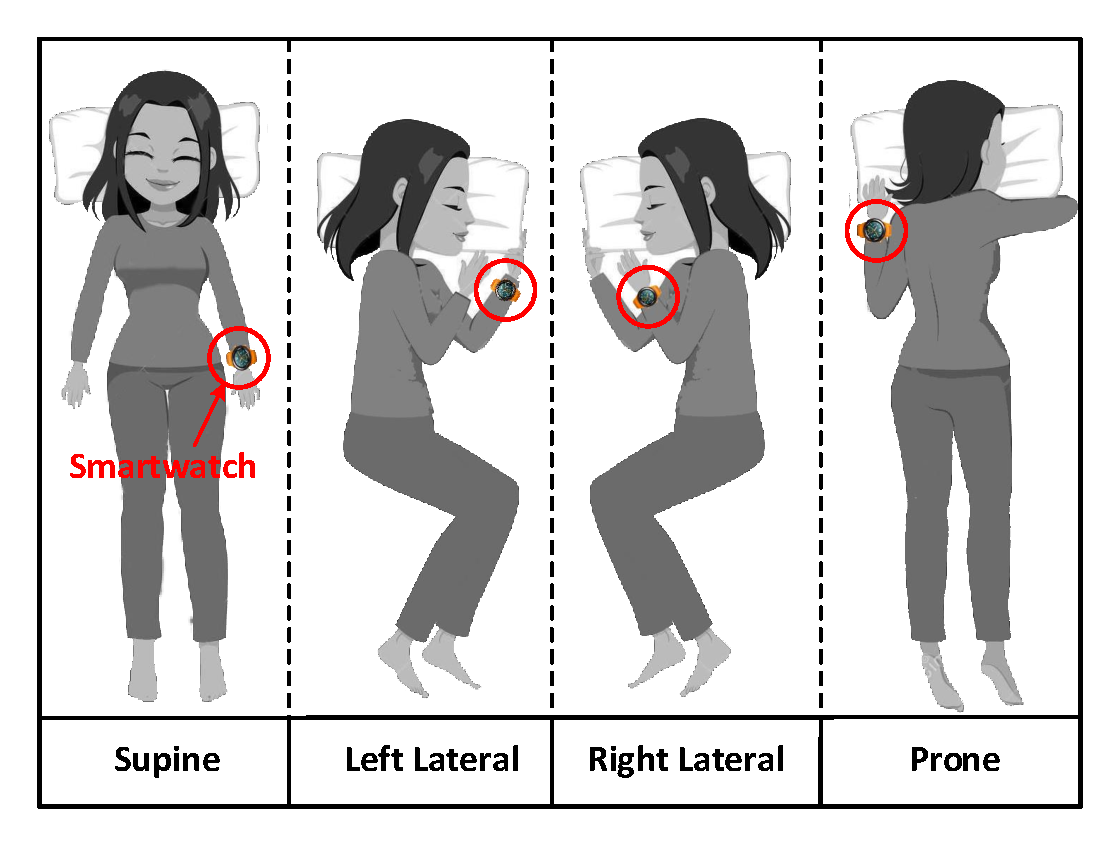
\includegraphics[width=0.87\linewidth]{Figures/BodyPosture.pdf}
  \caption{Four sleep body postures.}\label{fig:BodyPosture}
\end{figure}

\begin{figure}[!t]
  \centering
  \subfigure[Supine]{
    \label{fig:Supine}
    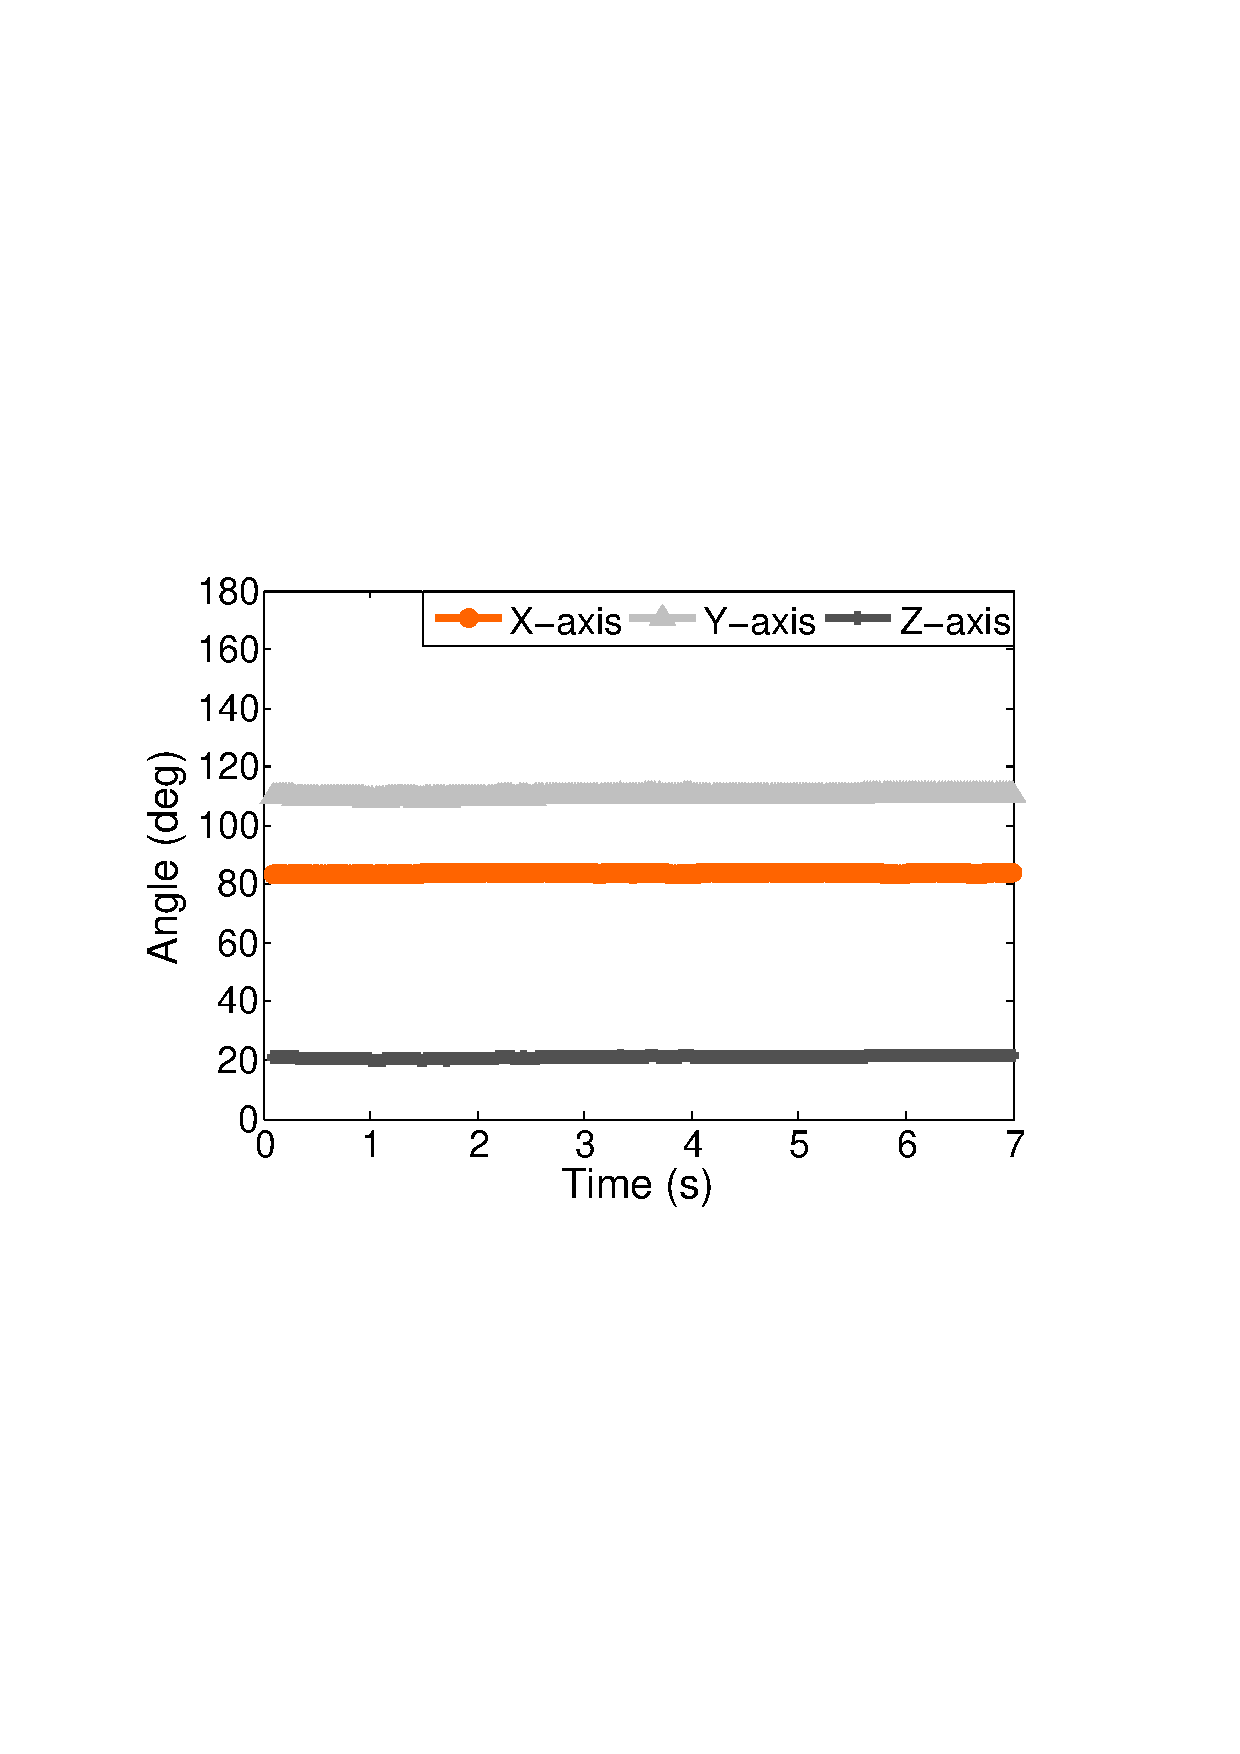
\includegraphics[width=0.47\linewidth]{Figures/Supine.pdf}}
  \hfill
  \subfigure[Left Lateral]{
    \label{fig:LeftLateral}
    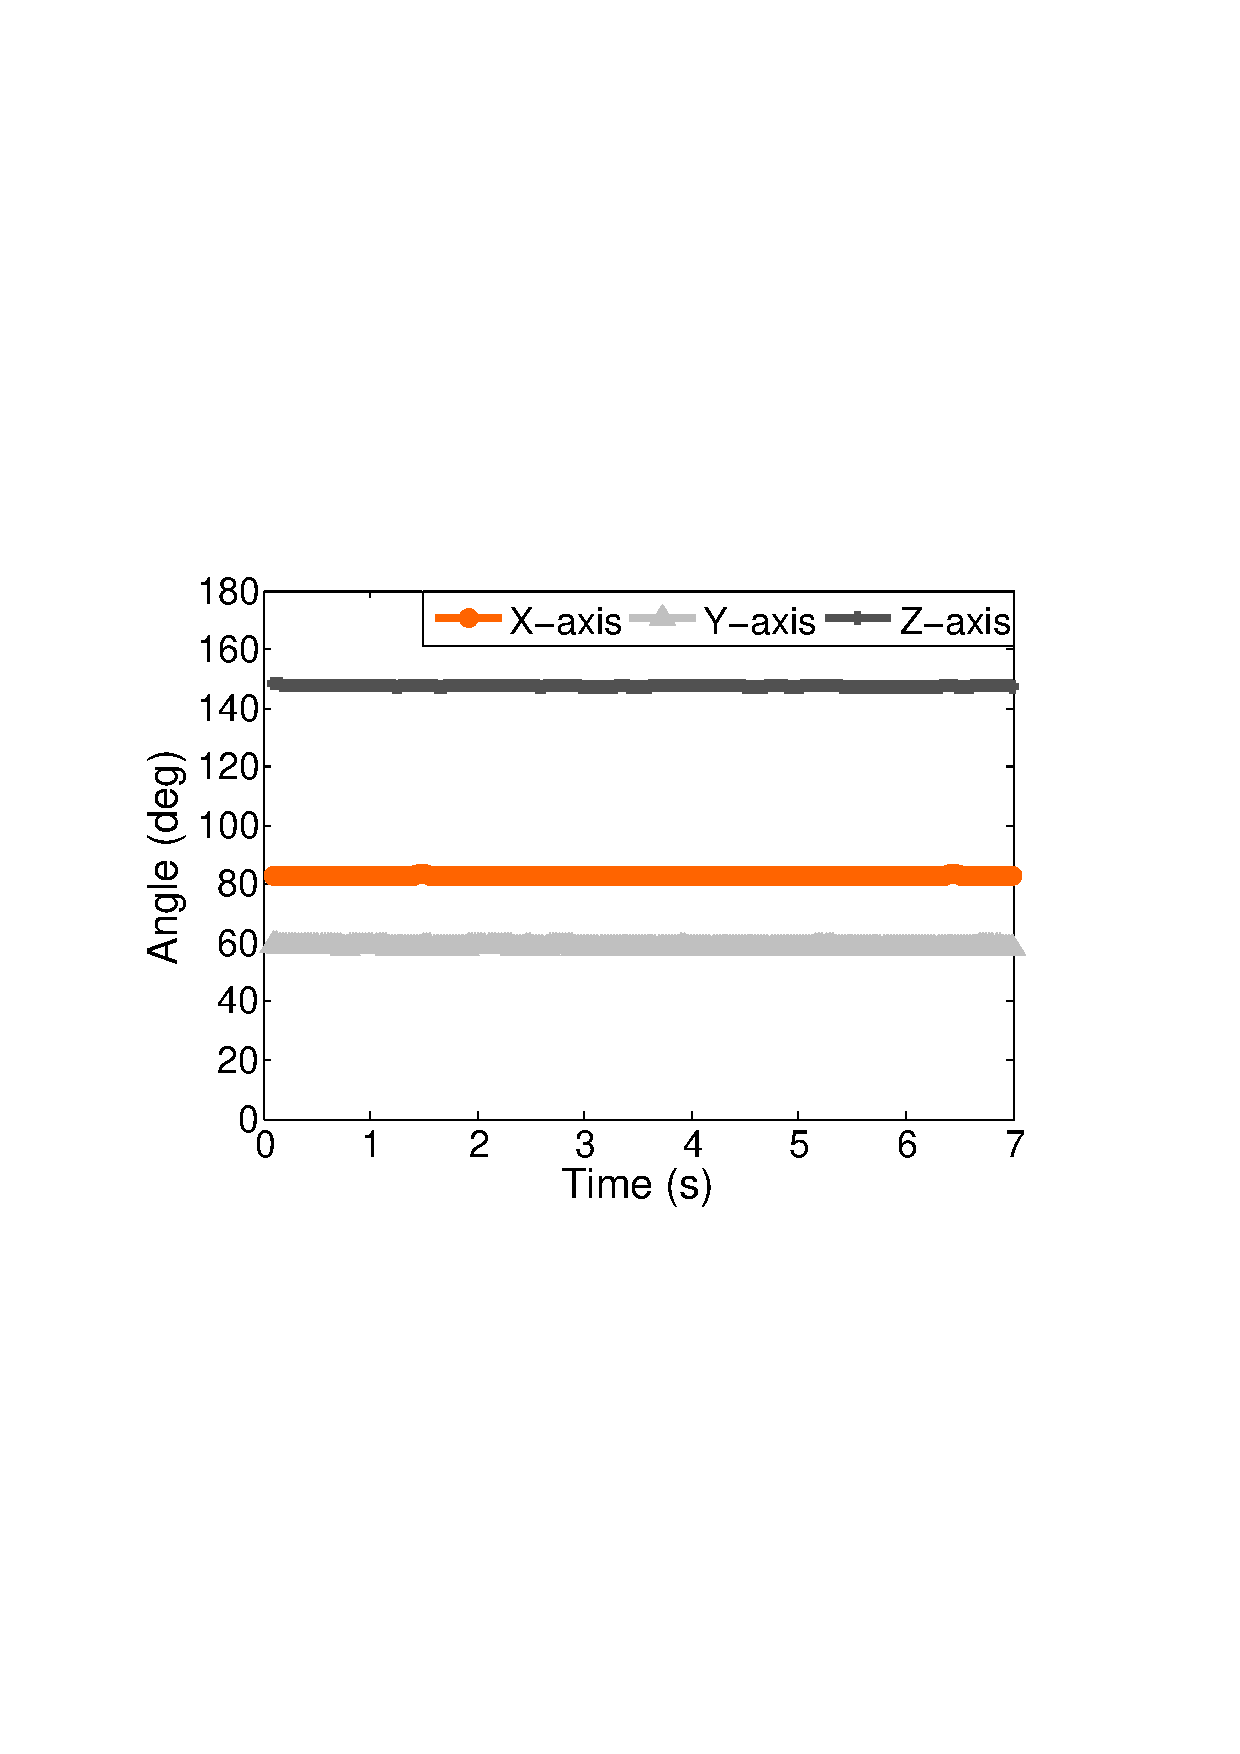
\includegraphics[width=0.47\linewidth]{Figures/LeftLateral.pdf}}
   \subfigure[Right Lateral]{
    \label{fig:RightLateral}
    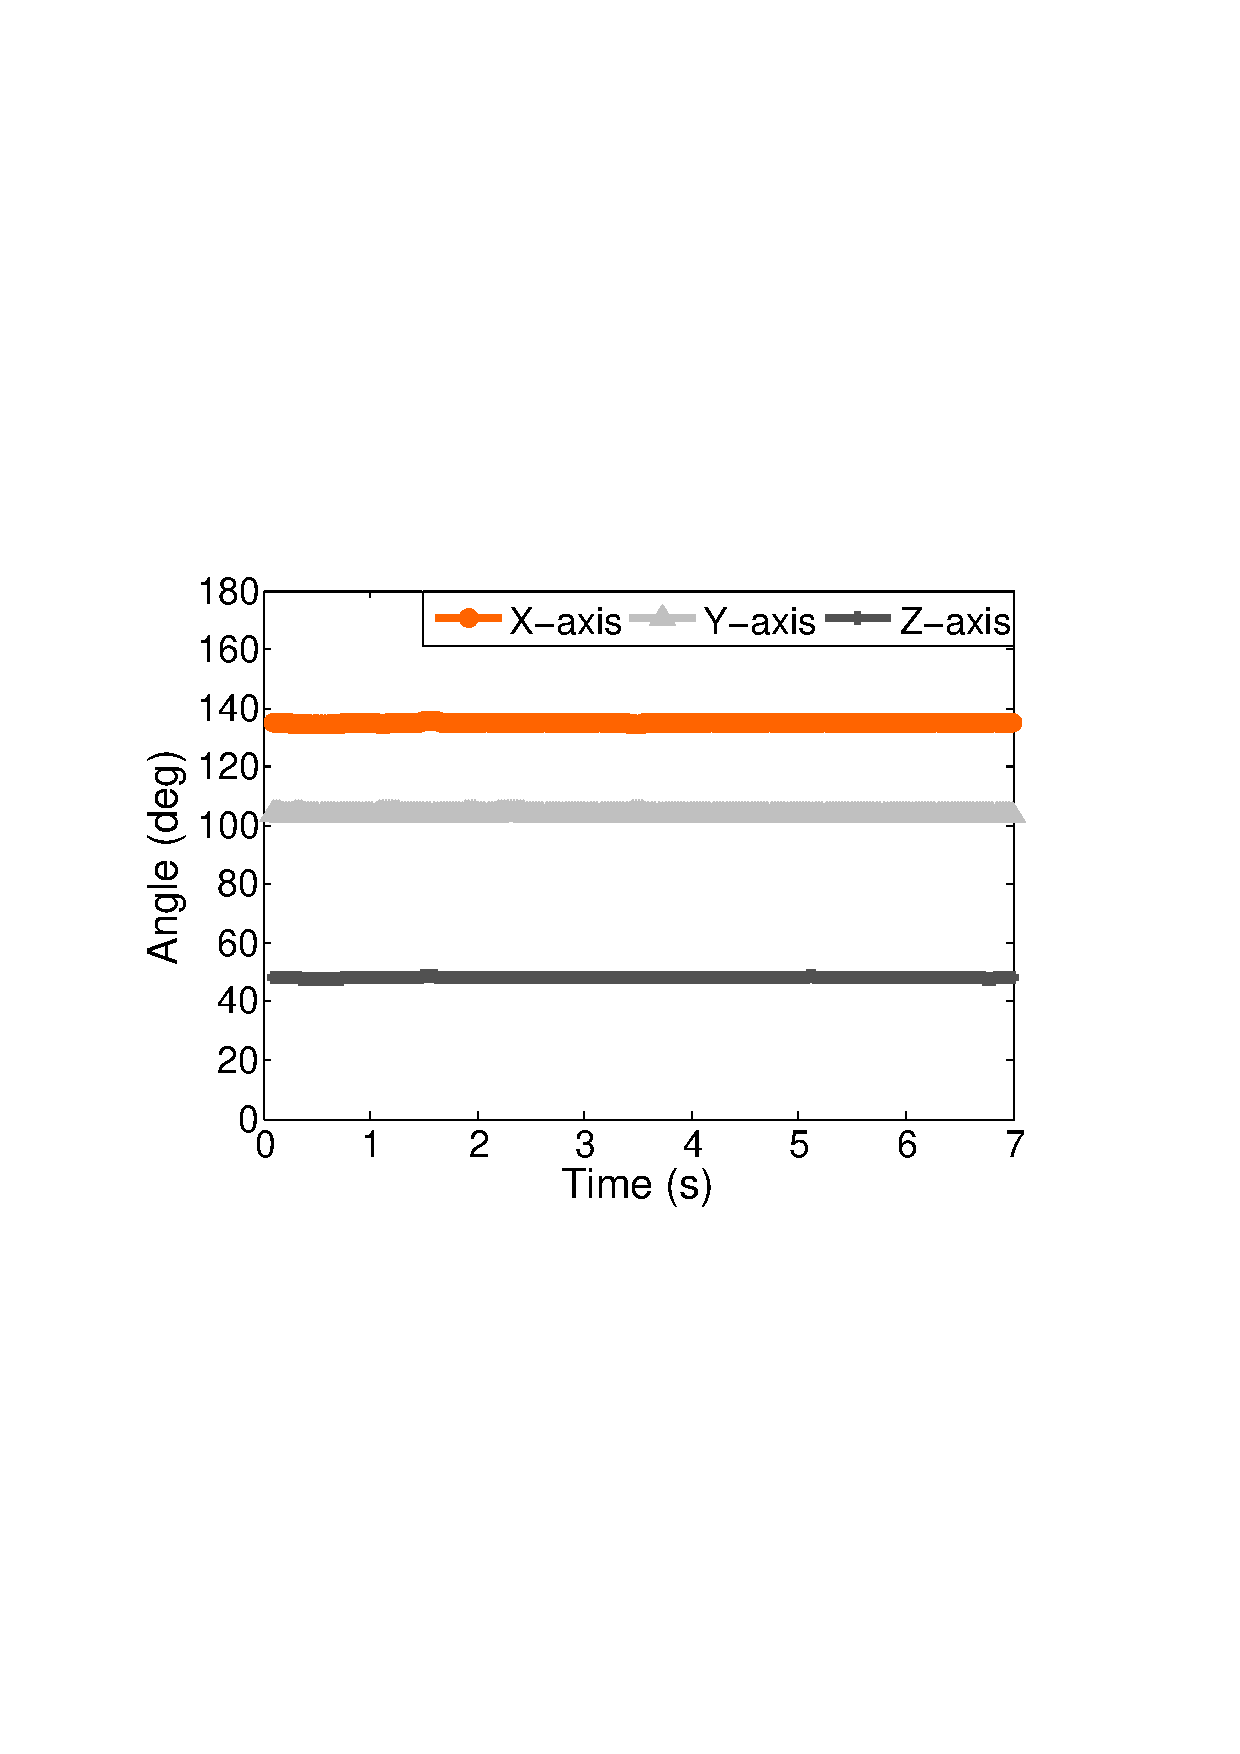
\includegraphics[width=0.47\linewidth]{Figures/RightLateral.pdf}}
  %\hspace{1in}
  \hfill
  \subfigure[Prone]{
    \label{fig:Prone}
    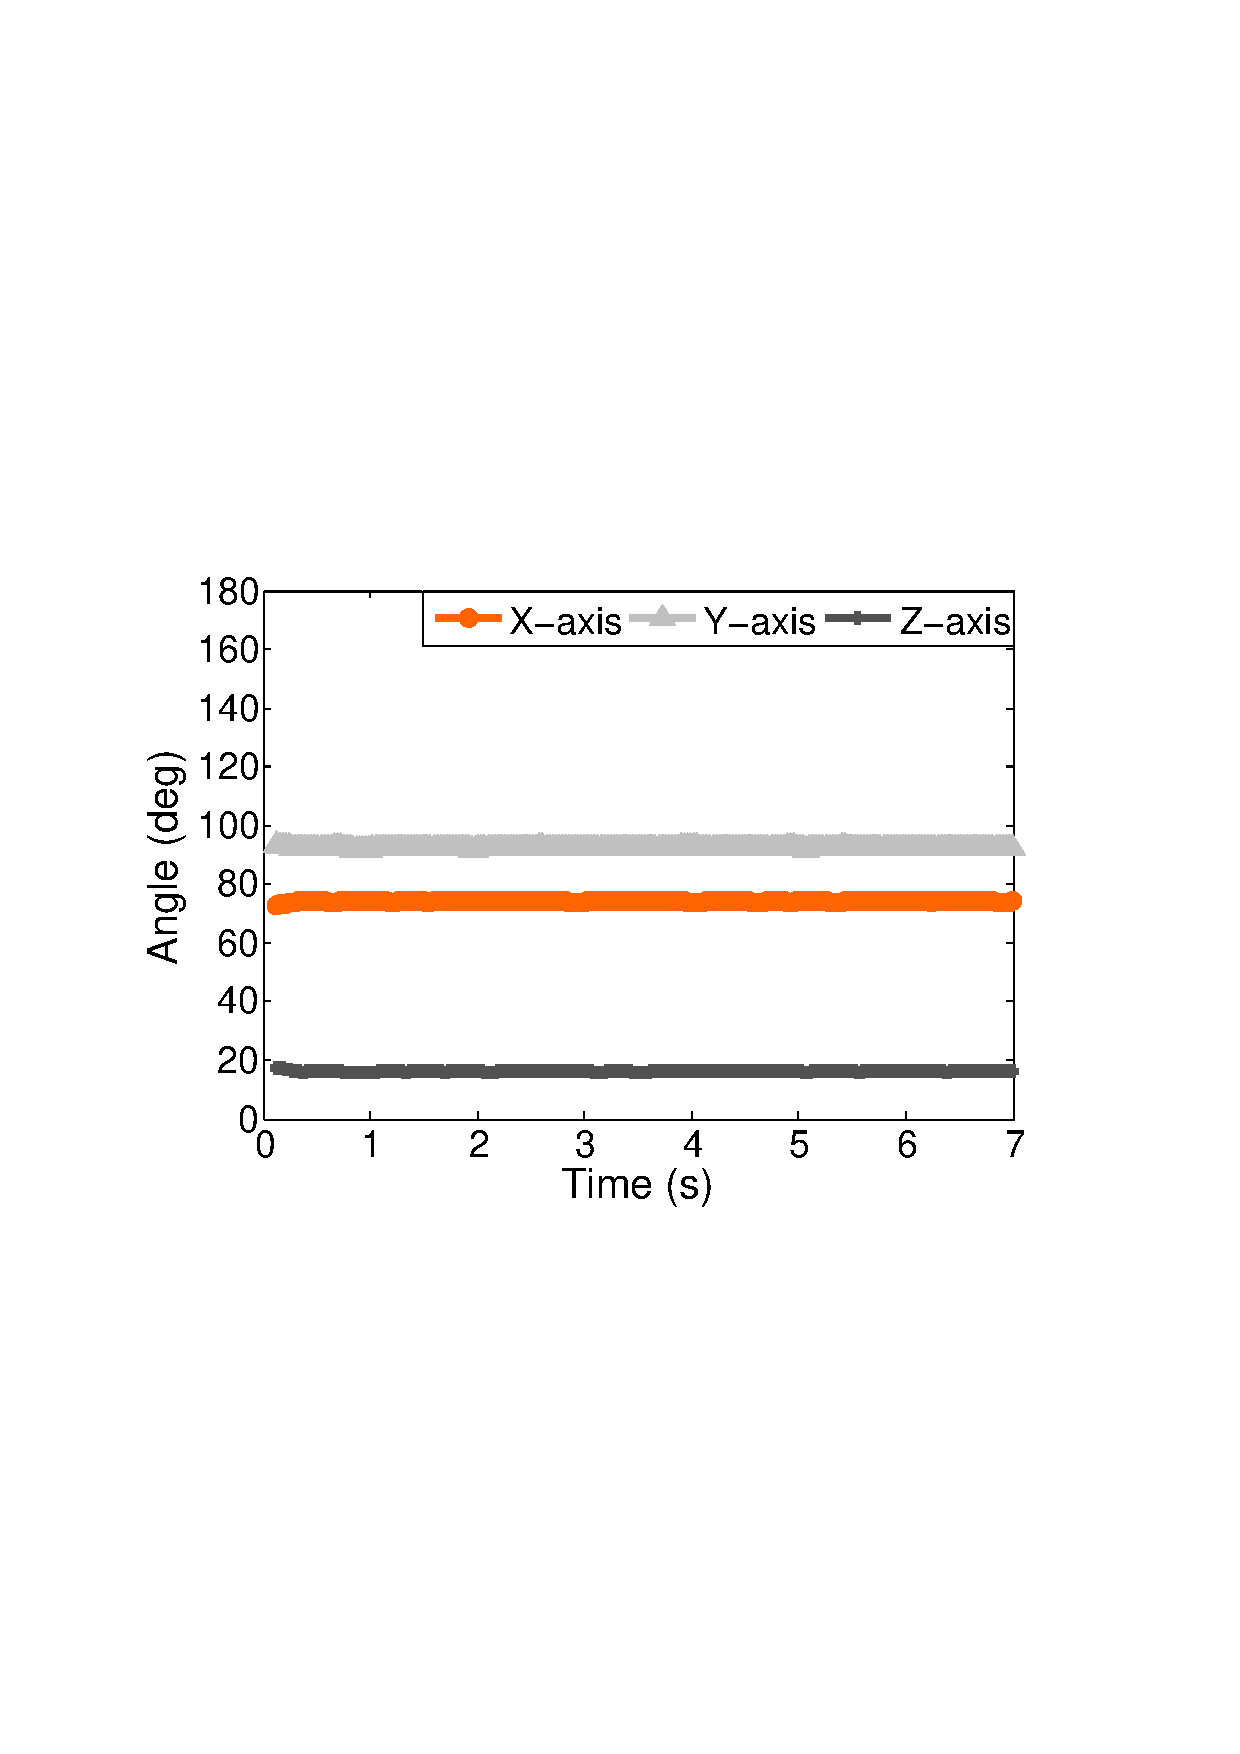
\includegraphics[width=0.47\linewidth]{Figures/Prone.pdf}}
  \caption{The tilt angle characteristics of four body postures.}
  \label{fig:posture}
\end{figure}

\subsection{Sleep Posture and Movement}
{\systemname} can monitor the user's sleep posture and habits, which is an indispensable factor of determining sleep quality and is heavily used in performing medical diagnoses \cite{oksenberg1998effect}. We present the detection details about the body posture and movement events. In {\systemname}, there are 4 different sleep postures, 3 different hand positions, 6 kinds of body rollover and 3 different micro body movements considered.  These events comprehensively and highly relates to the sleep stages and quality.

\textcolor{blue}{\subsubsection{Body posture detection}}
An effective posture detection and timely posture change can improve the sleep quality and sometimes the obstructive sleep apnea. We concentrate on four common body postures, that are supine, left lateral, right lateral and prone. According to our survey, most people's arms have some usual and  fixed positions in these four different sleeping positions, namely the arm's position is related to the body posture, which is similar to the idea of the sleep posture detection in \cite{sleepmonitor}. In {\systemname}, we consider the following situations. when user sleep in supine, we consider that user's hand put on the left sides of the body, on the abdomen, on the chest or on the head; when user sleep on left, we consider that user's hand put close to the pillow; When user sleep on right, the hand on the chest, on the waist or close to the pillow are considered by our system; And the hand on the side of the head or above the head, we consider, when user sleep in the prone posture. In the future work, we will consider more of the arm's position. Fig. \ref{fig:BodyPosture} shows that one of a position of arm in four different sleep postures.

We can choose the three-axis tilt angle calculated from the acceleration data as the feature \cite{sleepmonitor}. And then we use a supervised learning method to create a sleep posture profile. Specifically, we collect training data to create a mapping (i.e., angle mapping) between the angles and the arm under different positions. In order to extract the window-based tilt angle features, we average all the calculated angles in a window. Fig. \ref{fig:posture} shows the characteristics of four sleep postures with, it indicates that the tilt angles of three axes have obvious differences.The sleep postures thus can be inferred based on the positions of the smartwatch and the created angle mapping. However, we found that the supine features when the hand on the left sides of the body are similar with the prone features when the hand on the side of the head (Fig. \ref{fig:Supine} and \ref{fig:Prone}), thus the classification accuracy will be affected.

In order to improve the detection accuracy between the supine posture and prone posture, we go further to introduce the orientation sensory data as an auxiliary feature. This is based on the observation that the hand directions in the supine and prone positions are different. When the result of the previous step is prone or supine, we combine the tilt angle with three axes data obtained from the direction sensor as a new feature, and classify these postures more accurately based on the template distance matching. The posture will be detected as the one in the template which has a minimum Euclidean distance to it. Noted that when we use the direction sensor, we must limit the pillow orientation remaining unchanged (in the experiment our pillow is placed on the north). In fact, this assumption can be easily satisfied since most people usually have fixed sleep directions.


\textcolor{blue}{\subsubsection{Hand position recognition}}
The hand position during sleep discloses some potential health problems and the improper hand position will bring bad results. For instance, the hand position on the abdomen may indicate its uncomfortable state, while the person is usually not aware of that cases; when the hand is put on the chest, the person is more likely to have a nightmare because of the long-term oppression on the heart; And when the hand is put on the head, it can put excess pressure on the nerves in your shoulders, shoulder and arm pain is quite common, as blood flow is restricted in this position. This can lead to eventual nerve damage, with symptoms including a tingling sensation and numbness \cite{position2014}. {\systemname} can recognize three hand positions, that are on the abdomen, chest or head when the user is in the supine posture, as shown in Fig. \ref{fig:HandPosition}. Note that because in other body postures, the hand is put on the bed at most time, thus we do not consider different hand positions when the body are in other postures.

\begin{figure}[!t]
\centering
      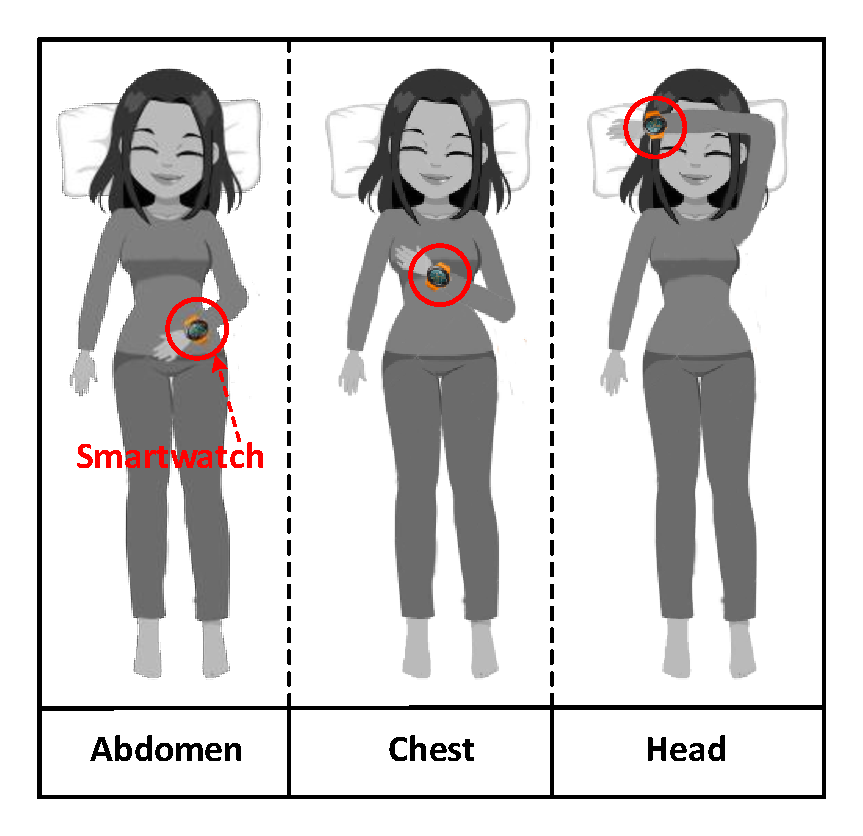
\includegraphics[width=0.7\linewidth,height=4.8cm]{Figures/HandPosition.pdf}
  \caption{Three hand positions.}\label{fig:HandPosition}
\end{figure}


In fact, when people are sleeping in the supine posture, the hands may be on both sides of the body, on the abdomen, chest or head. To identify the hand position accurately, we present a new algorithm based on our key observation. We have observed that before the hand put on the body initially, it usually experiences a movement from the body side to the end position, and after that the hand always experiences a movement from one position to the other. Thus we can further integrate the hand movement trajectory to determine the hand position at current time. In {\systemname}, We consider nine kinds of the trajectories of hand, from the side of the body to the abdomen, to the chest, to the head; from the chest to the abdomen, to the head; from the abdomen to the chest, to the head; from the head to the abdomen, to the chest. Fig. \ref{Bodyhand} shows the rotation angle changes when the hand is moving from the body side to different positions on the body. We use the three-axis rotation angle calculated by the gyroscope as a feature to establish a sample library, and use the template distance matching classifier to identify the final position of the hand.


According to the trajectory of hand movement can roughly determine the shot in the head, or in the part close to the chest, or in the part near the abdomen. However, depending on the trajectory, we can not be sure that the hand is exactly in the chest or abdomen. This is because when the hand move to the shoulder or hip and some other areas close to the chest or abdomen, we can know that the trajectories of the hand are very similar, so we need to go further to determine the hand on the chest or abdomen. Obviously, when the hand is put on the abdomen or chest, we can see that the acceleration signals exhibit a distinctly periodic fluctuation, as shown in Fig. \ref{Bodyhand}. This is due to the movement of the abdomen and chest caused by breathing.Therefore, we can use the occurrence of respiratory events to determine if the hand is indeed on the body (abdomen or chest). Specifically, we calculate the power spectral density (PSD) of the acceleration signal, where the highest peak frequency is the signal's frequency. From Fig. \ref{fig:PSD}, we can see that there is a large peak located at around 0.25 Hz, which corresponds the respiratory frequency. So if the signal's frequency falls within the reasonable breathing frequency range, which is around 20 times per minute (0.3 Hz), it indicates the occurrence of respiration events, that is, the hand is put on the chest or abdomen.

In addition, we found that the extent of body movements can be used to judge the amplitude of respiration. What's more, we know that when people sleep in the REM stage, they respiratory amplitude smaller than the respiratory amplitude sleep in the NREM stage \cite{respiratory1982}, so we can roughly determine the user's current sleep stage based on the respiratory amplitude. Of course, respiratory amplitude is only an indicator of the division of the sleep stage, we can not regard it as a basis for final judgment, only for reference here and it can help later division of the sleep stage. Under normal circumstances, the chest movement amplitude is smaller than abdominal movement amplitude. However, in different sleep stages, the respiration amplitudes are different \cite{respiratory}. It is likely that there is a situation: the chest movement amplitude in the NREM sleep stage is close to the abdominal movement amplitude in the REM sleep stage. As a result, the threshold based method cannot work. At this time, we need to combine it with the position of the hand we detected with the trajectory before. Through the above steps, we have been able to determine whether the hands are on the chest or abdomen, and then we can go further to determine the extent of breathing according to the degree of body ups and downs, and we can roughly infer the sleep stage. Now we take the case of hands on the abdomen as an example.

\begin{figure}[!t]
  \centering
   %\begin{minipage}[t]{0.325\linewidth}
  \subfigure[]{\label{BodytoAbdomen}
   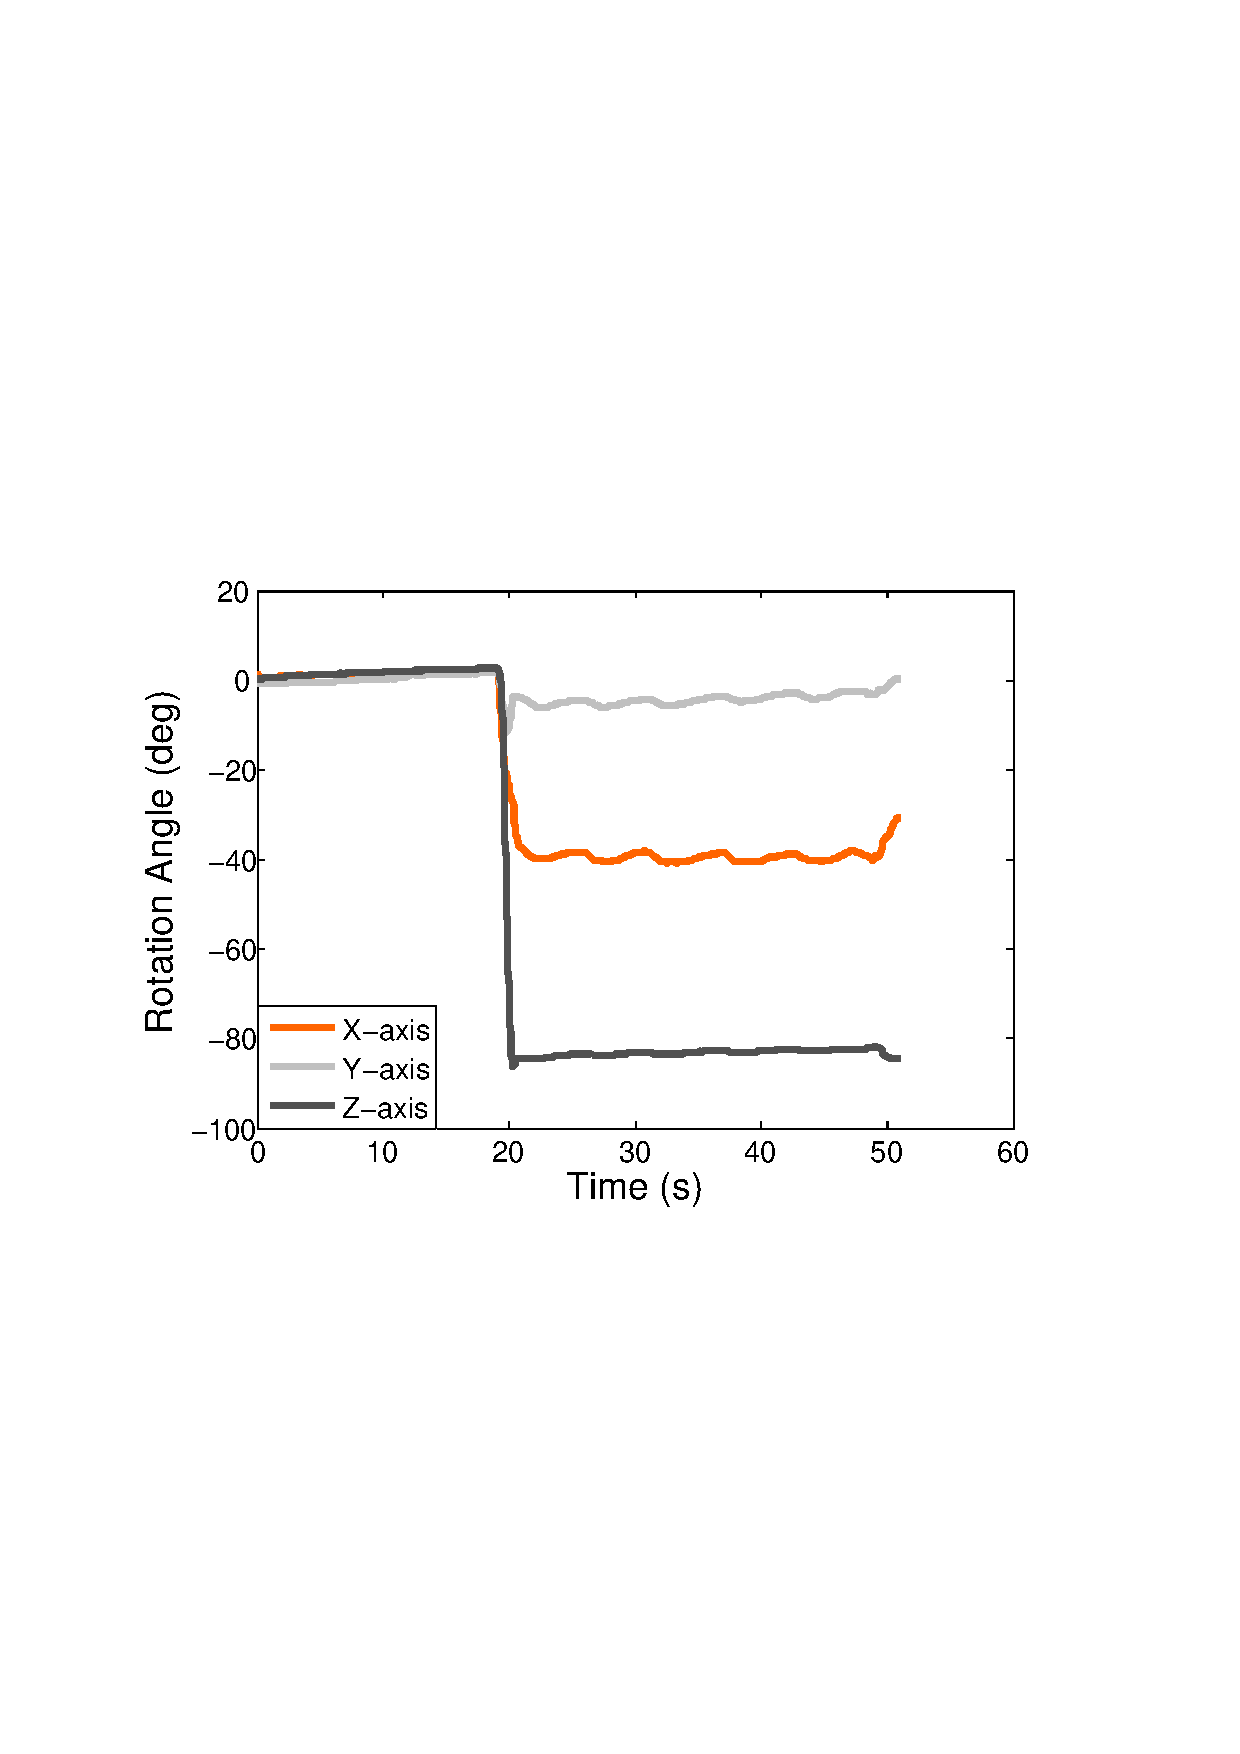
\includegraphics[width=2.7cm,height=2cm]{Figures/BodytoAbdomen.pdf}}
%  \hfill
   \subfigure[]{\label{BodytoChest}
   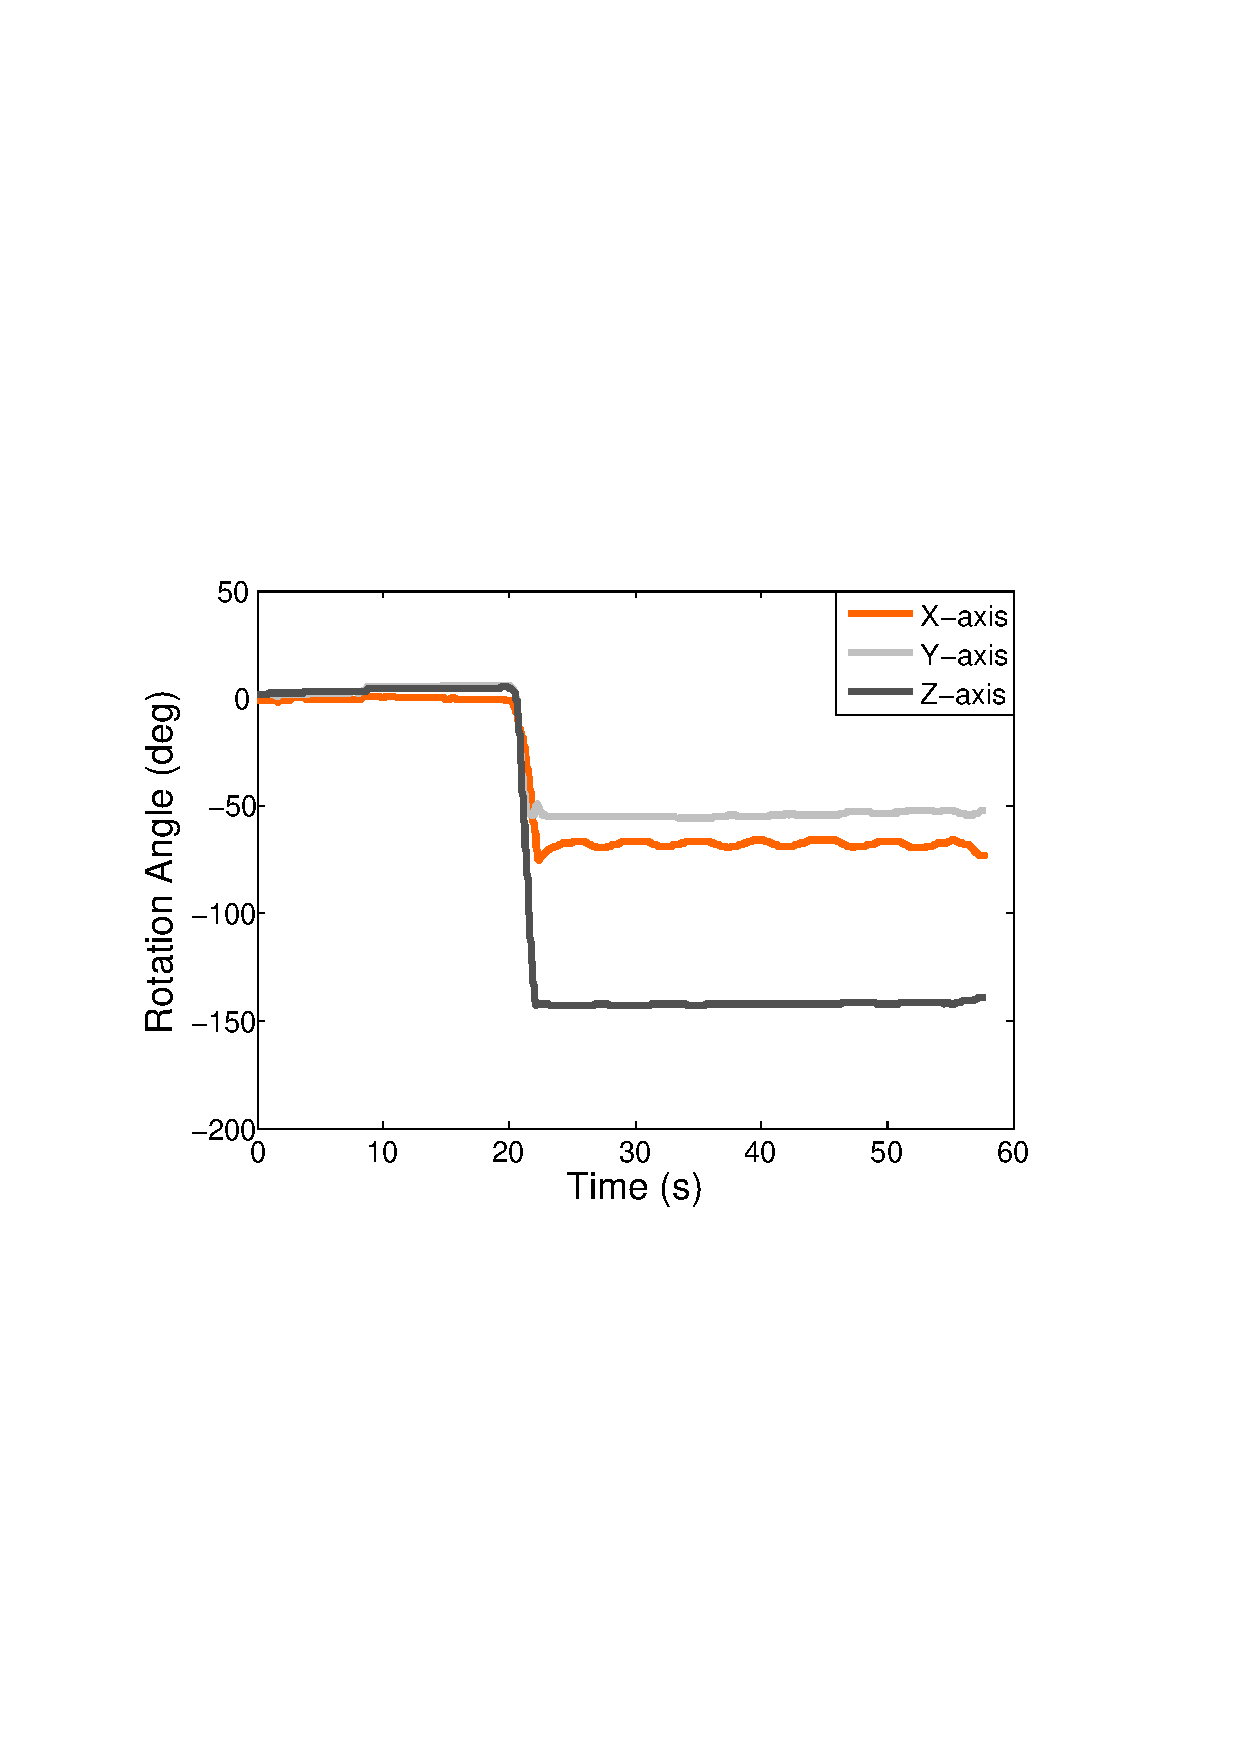
\includegraphics[width=2.7cm,height=2cm]{Figures/BodytoChest.pdf}}
%  \hfill
  \subfigure[]{\label{BodytoHead}
   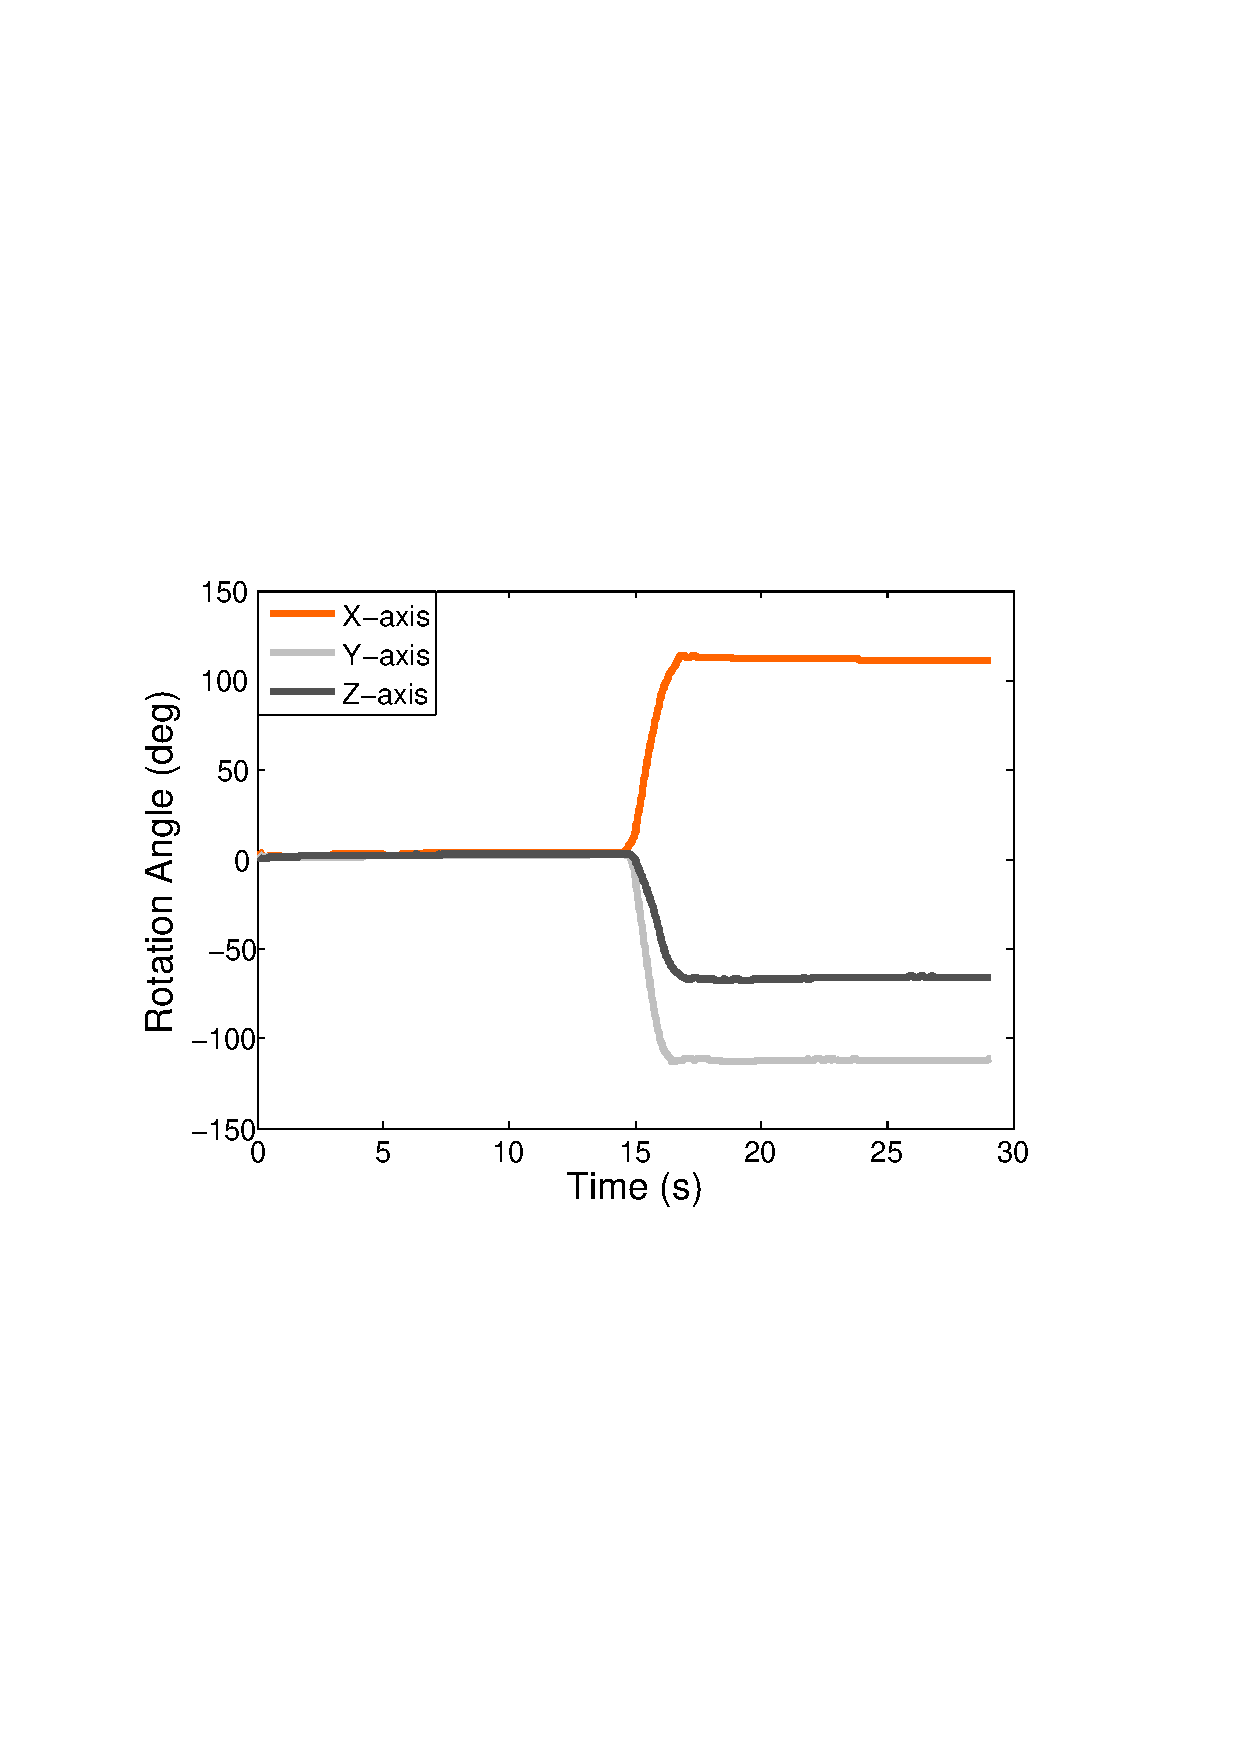
\includegraphics[width=2.7cm,height=2cm]{Figures/BodytoHead.pdf}}
   \caption{The characteristics of hand movement from the position beside the body  to (a)  the abdomen,  (b) the chest, and (c) the head.}\label{Bodyhand}
\end{figure}

\begin{figure}[!t]
\centering
      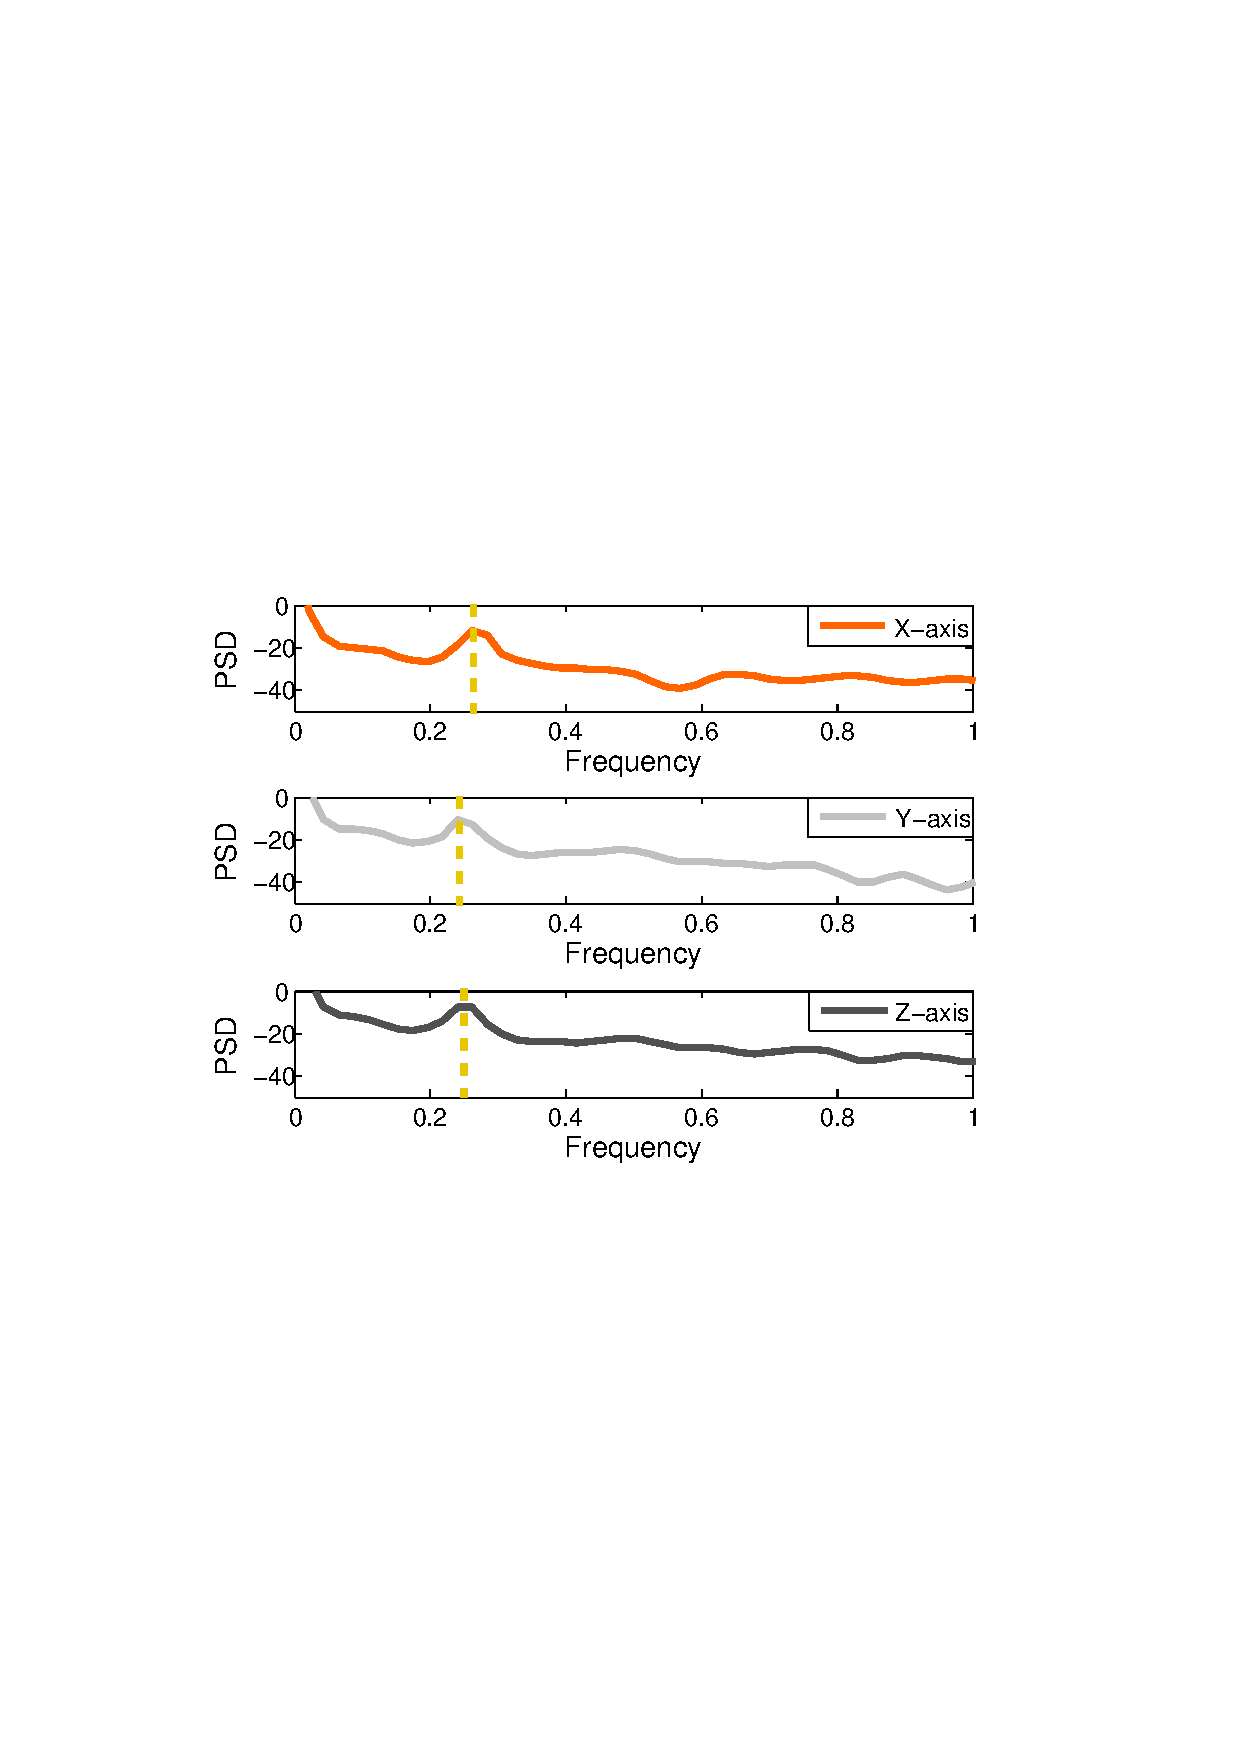
\includegraphics[width=0.77\linewidth]{Figures/PSD.pdf}
  \caption{The power spectral density (PSD) of the acceleration signal.}\label{fig:PSD}
\end{figure}

\begin{figure}[!t]
\centering
      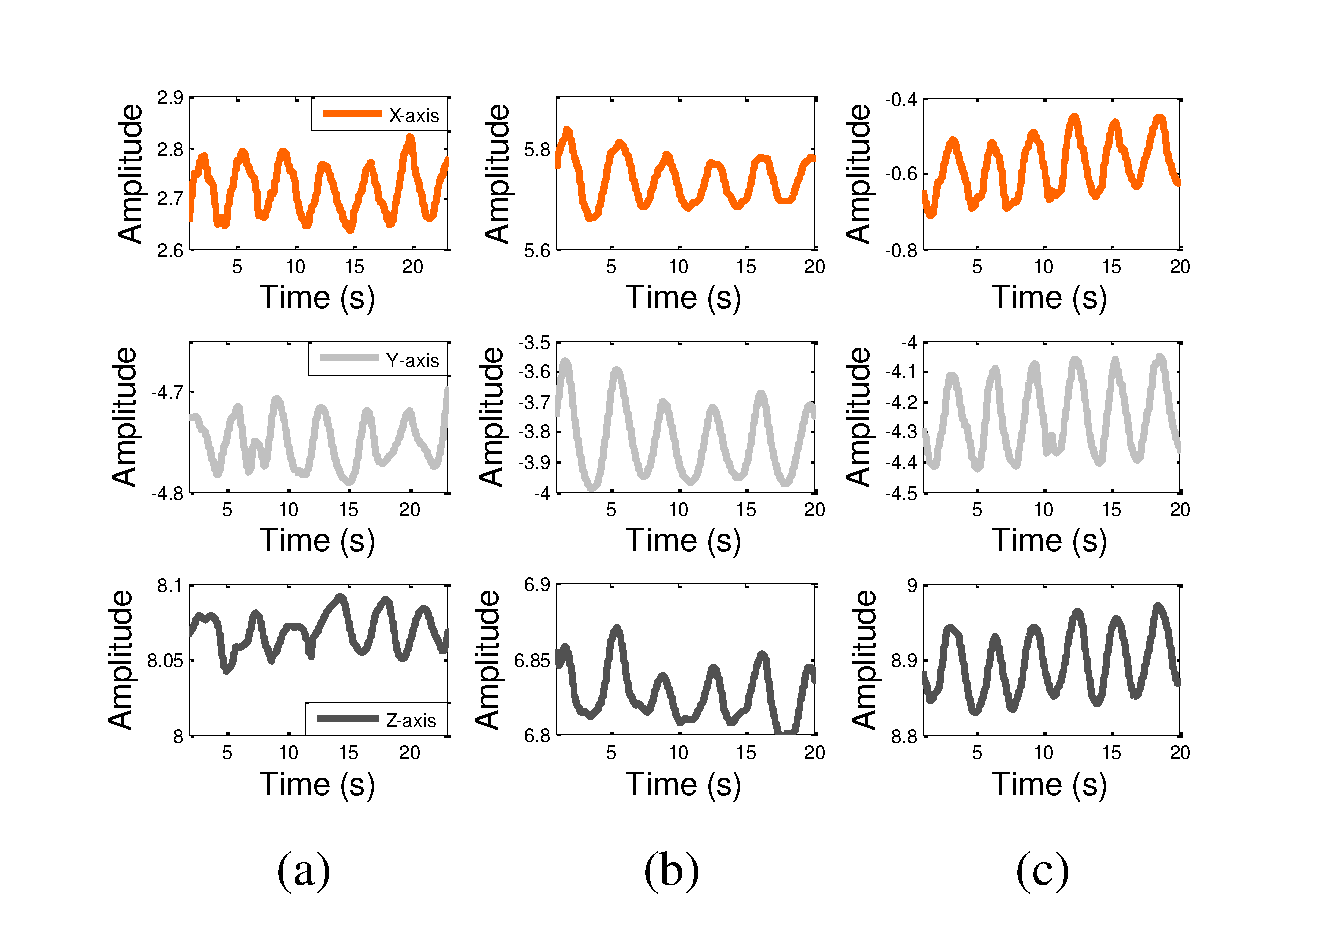
\includegraphics[width=0.77\linewidth]{Figures/breath_ok1.pdf}
  \caption{The periodic change of the acceleration signal. (a) REM--Location 1. (b) REM--Location 2.  (c) NREM--Location 1.}\label{fig:breath_ok1}
\end{figure}

In detail, we found that even the abdomen position, due to the specific location of user's hand put a little different every time, it makes the position of the smartwatch is different, the intensity of the acceleration fluctuation caused by respiration along each axis may be different, so we can not use the direct measured amplitude information to determine respiratory amplitude, as shown in Fig. \ref{fig:breath_ok1}, (a) and (b) are triaxial accelerations at different locations of the abdomen during REM sleep stage, and (c) is the acceleration data of NREM sleep stage at the approximate position in (a). We can see that when hand on the abdomen, but the location is different, even in the same location, we can not directly judge the respiration amplitude using only the amplitude of the acceleration.

\begin{figure}[!t]
\centering
      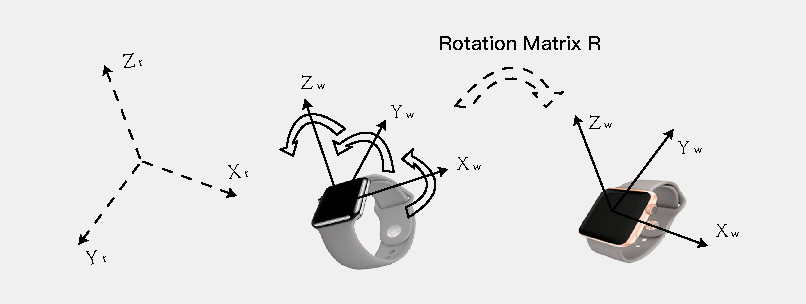
\includegraphics[width=0.97\linewidth]{Figures/watch.pdf}
  \caption{The first figure on the left is the body coordinate system, and $Y_t$ points north. The middle figure shows the watch coordinate system when the watch an arbitrary position, and the right of the figure shows that the  watch coordinate system after we completed the coordinate system conversion.}\label{fig:watch}
\end{figure}

In order to solve this problem, we decided to convert the acceleration data based on the wristwatch coordinate system into the data in the world coordinate system. As shown in Fig. \ref{fig:watch}, the watch coordinate system ({[$X_w$, $Y_w$, $Z_w$]}) is determined by the position of the watch. Our coordinate alignment aims to find a rotation matrix R to convert the watch's coordinate system to the torso coordinate system ({[$X_t$, $Y_t$, $Z_t$]}). We express the triaxial acceleration data as $Acc_w$ = [$X_w$, $Y_w$, $Z_w$] in the wristwatch coordinate system and Acct = [$X_t$, $Y_t$, $Z_t$] in the torso coordinate system, and R can be obtained by the three-axis direction information in the orientation sensor.

\begin{equation}
      X_��=(X_w\cos\gamma + Y_w\sin\gamma)\cos\theta + (Y_w\cos\sigma + Y_w\sin\sigma)\sin\theta,
\end{equation}
\begin{equation}
     Y_��=-((Y_w\cos\sigma + Y_w\sin\sigma)\cos\theta - (X_w\cos\gamma + Y_w\sin\gamma)\sin\theta),
\end{equation}
\begin{equation}
     Z_��=(Z_w\cos\gamma - Z_w\sin\gamma)\cos\theta - (Z_w\cos\gamma - Z_w\sin\gamma)\sin\theta,
\end{equation}

$\theta$, $\sigma$ and $\gamma$ are the x, y and z axis data of the orientation sensor respectively, representing the direction angle, the tilt angle and the roll angle collected from the orientation sensor. After the alignment of the coordinate system, we can see from Fig. \ref{fig:cordi} that the z-axis shows a periodic signal with significant fluctuations, while the x- and y-axis data undergo smaller changes around zero, which is consistent with the actual situation that when the person is in the supine posture with the abdomen up and down caused by respiratory.

 \begin{figure}[!t]
\centering
      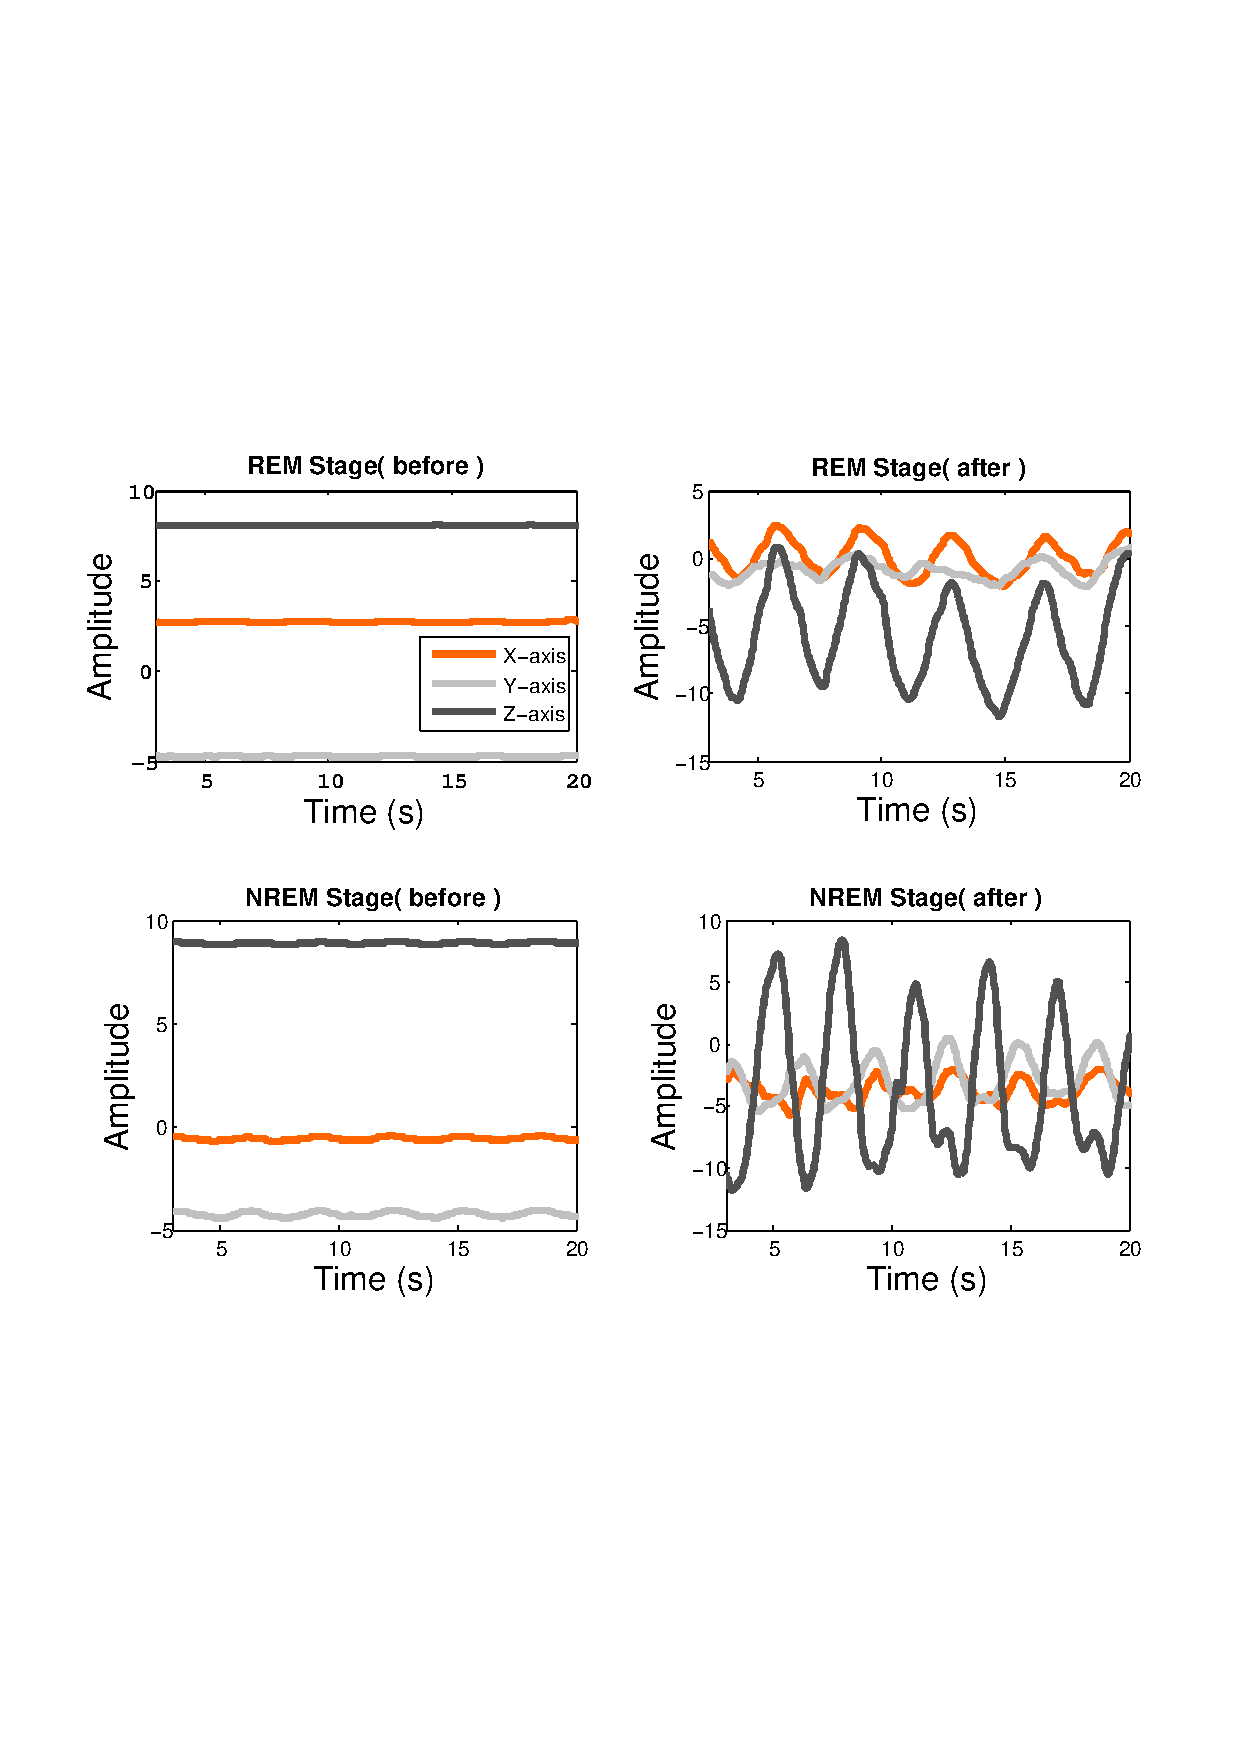
\includegraphics[width=0.97\linewidth]{Figures/cordi.pdf}
  \caption{Acceleration data for different sleep stages.}\label{fig:cordi}
\end{figure}

The two graphs on the left in Fig. \ref{fig:cordi} show the acceleration data in (a) and (c) in Fig. \ref{fig:breath_ok1}, respectively, and the two graphs on the right are these data after the conversion of the coordinate system. We can see that before the alignment of the coordinate system, we can not effectively distinguish between REM stage and NREM stage respiratory amplitude from the acceleration amplitude, but after the coordinate system alignment, we can judge the amplitude from the z-axis data well. Here, we choose to calculate the amplitude variances of the z-axis acceleration as a feature, it can be used to measure the intensity of the fluctuation in a signal and a larger variance means that the greater the amplitude of the breaths. Therefore, we further train the variance of the acceleration data when the hand on the abdomen and on the chest under the REM stage and the NREM stage to determine the current respiratory amplitude. We trained 200 sets of acceleration data (100 sets of these from the larger respiratory amplitude and the rest of sets from the normal respiratory amplitude ) from 10 volunteers. Eventually, we concluded that the variance threshold for the acceleration data is 15 when the hand on the abdomen, and the variance threshold is 4 when the hand on the chest.


 \begin{figure}[!t]
\centering
      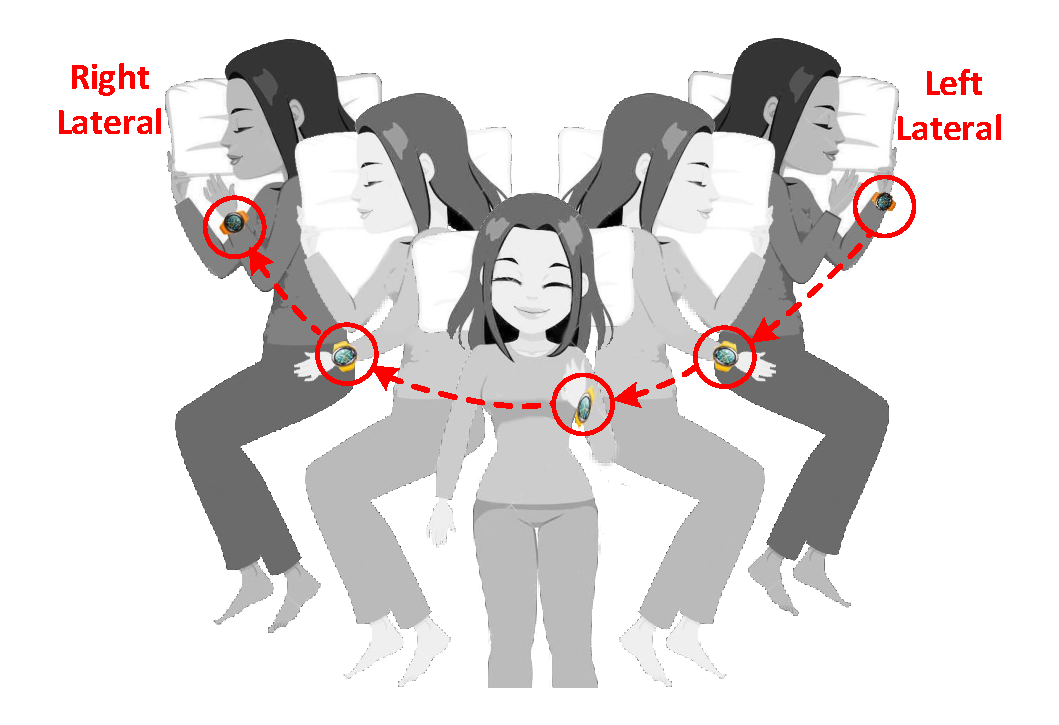
\includegraphics[width=0.77\linewidth]{Figures/BodyRollover.pdf}
  \caption{Body rollover from the left side to the right side.}\label{fig:BodyRollover}
\end{figure}


\textcolor{blue}{\subsubsection{Body rollover counts}}
Under normal circumstances, people usually body rollover about 20-45 times a night, the meaning of body rollover is to maintain a comfortable position. Otherwise, for a long time to maintain a sleep posture, some muscles will be in a state of tension, making the body in contact with the bed due to oppression caused by poor blood supply, nerve compression will lead to local numbness \cite{rollover2014}. So body rollover is another key indicator about the sleep quality. {\systemname} can detect the number of body rollovers. In general, there are six cases: four posture transition cases between the supine posture and lateral (left or right) posture, and two posture transitions between the left lateral posture and right lateral posture. Fig. \ref{fig:BodyRollover} shows the case when the body moves from the left side to the right side. When the rollover occurs, we observe different change patterns about the tilt angle values. Specifically, the angle values of three different axes are on the falling edge or rising edge simultaneously during a very short time period. Fig. \ref{fig:LeftToRight} -- Fig. \ref{fig:RightToLeft} shows the value changes under different body rollover cases. To this end, one straightforward method to detect the rollover is to test the angle value changes. However, this method suffers a very large error since other hand movements will also induce a similar data changes.

\begin{figure*}[!t]
%\centering
%   \setlength{\abovecaptionskip}{-2pt}
% \setlength{\belowcaptionskip}{-9pt}
\begin{minipage}[t]{0.31\linewidth}\centering
    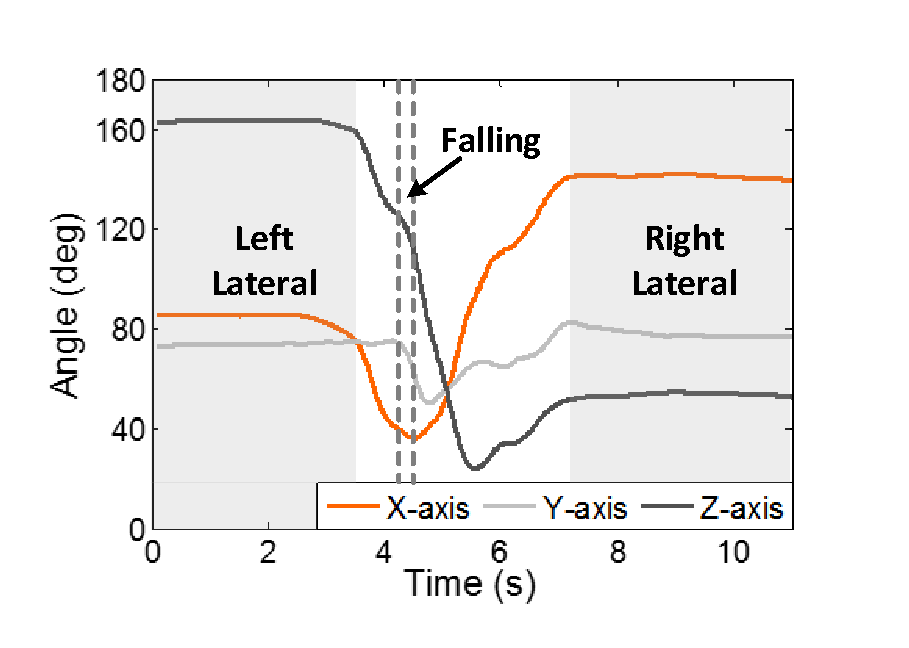
\includegraphics[width=0.97\linewidth,height=3.7cm]{Figures/LeftToRight.pdf}\centering
  \caption{From left lateral posture to right lateral posture.}\label{fig:LeftToRight}
\end{minipage}
\hspace{2pt}
\begin{minipage}[t]{0.31\linewidth}\centering
    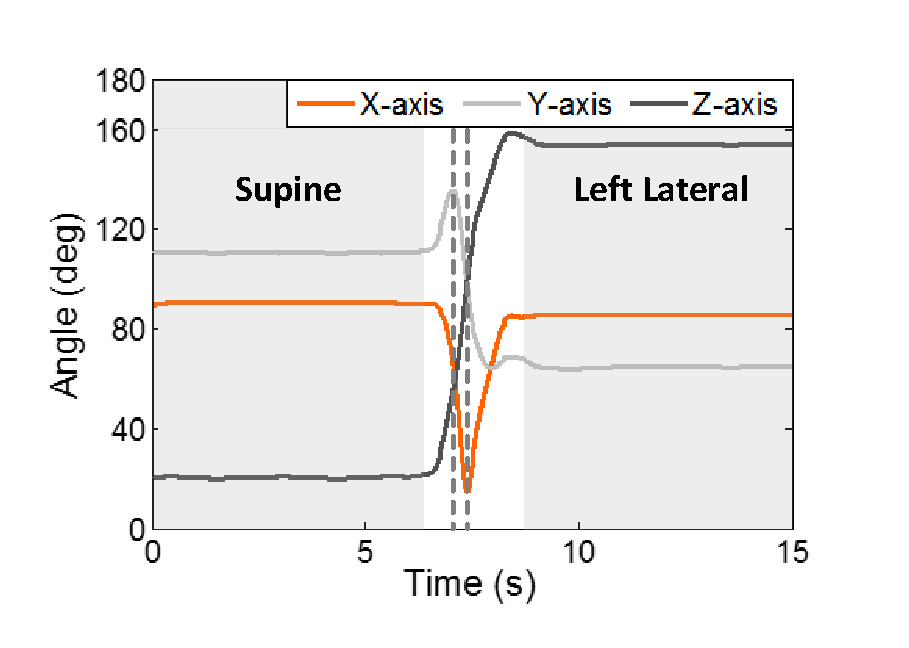
\includegraphics[width=0.97\linewidth,height=3.7cm]{Figures/SupineToLeft.pdf}\centering
  \caption{From supine posture to left lateral posture.}\label{fig:SupineToLeft}
\end{minipage}
\hspace{2pt}
\begin{minipage}[t]{0.31\linewidth}\centering
    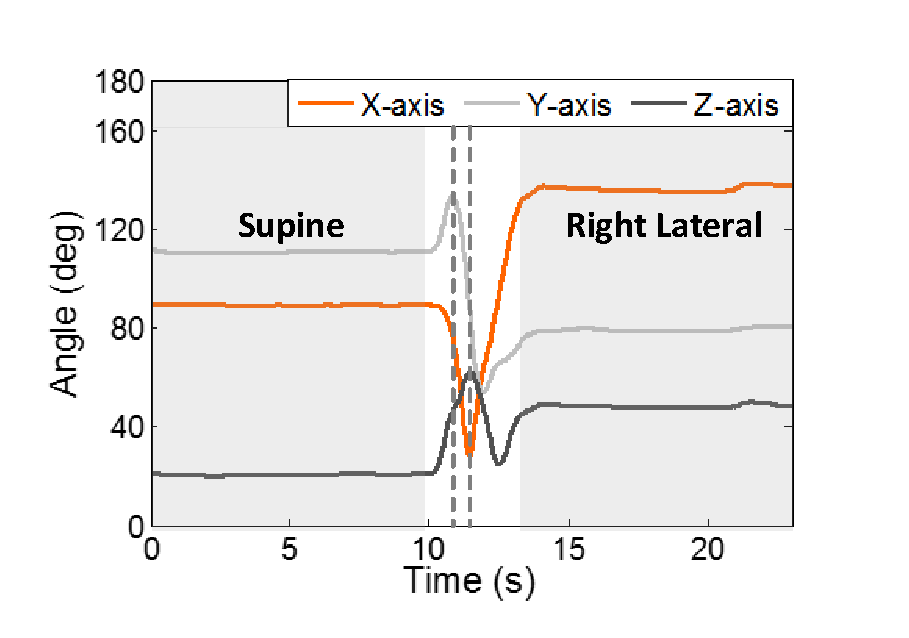
\includegraphics[width=0.97\linewidth,height=3.7cm]{Figures/SupineToRight.pdf}
  \caption{From supine posture to right lateral posture.}\label{fig:SupineToRight}
\end{minipage}
\hspace{5pt}
\begin{minipage}[t]{0.31\linewidth}\centering
    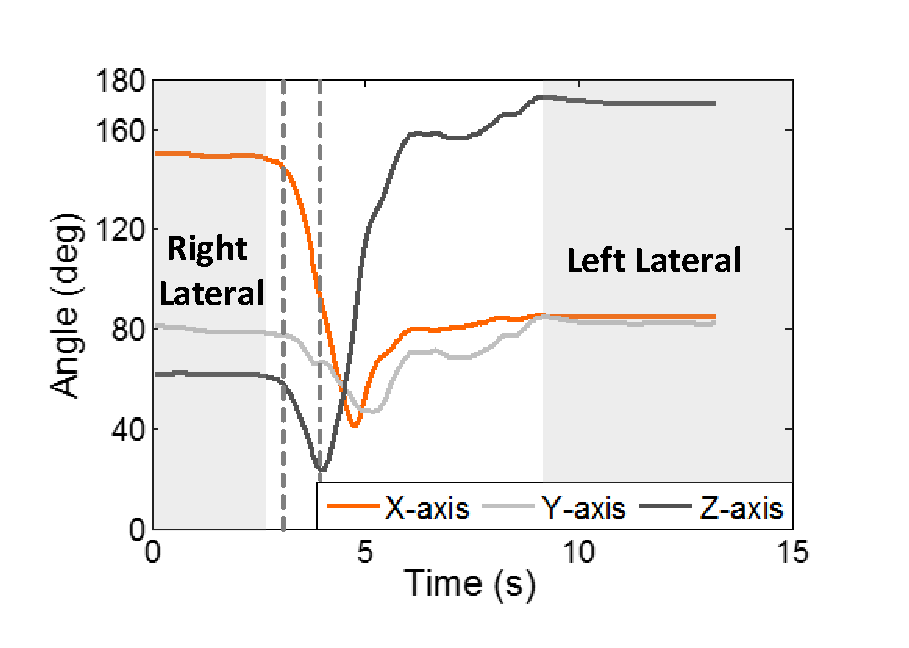
\includegraphics[width=0.97\linewidth,height=3.7cm]{Figures/RightToLeft.pdf}
  \caption{From right lateral posture to left lateral posture.}\label{fig:RightToLeft}
\end{minipage}
\hspace{12pt}
\begin{minipage}[t]{0.31\linewidth}\centering
    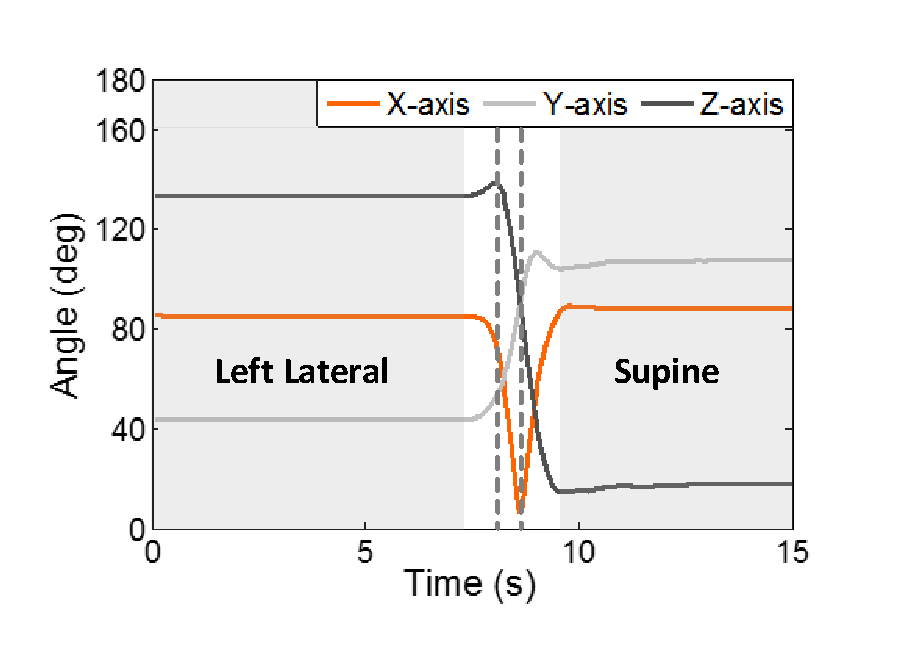
\includegraphics[width=0.97\linewidth,height=3.7cm]{Figures/LeftToSupine.pdf}
  \caption{From  left lateral posture to supine posture.}\label{fig:LeftToSupine}
\end{minipage}
\hspace{16pt}
\begin{minipage}[t]{0.31\linewidth}\centering
    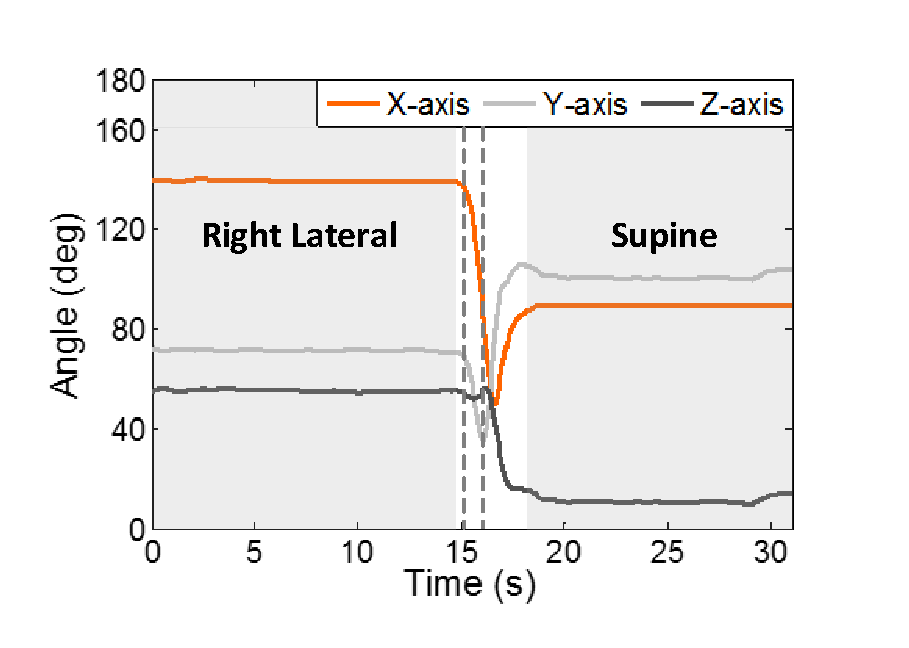
\includegraphics[width=0.97\linewidth,height=3.7cm]{Figures/RightToSupine.pdf}\centering
  \caption{From right lateral posture to supine posture.}\label{fig:RightToLeft}
\end{minipage}
\end{figure*}

To deal with this challenge, we incorporate the body postures to improve the detection accuracy. As shown in Fig. \ref{fig:BodyRollover}, the body postures are different before and after the rollover. Therefore, after we detect the time when the angle values changes, we term the time as a possible rollover time point. Then we use the sleep posture classification algorithm to determine whether the body postures are the same or not over a period of time before and after this point. If the postures are different, we exclude this time point, otherwise the system detects a body rollover event. Note that {\systemname} can not only count the number of rollovers, but also report the detailed rollover event.


\textcolor{blue}{\subsubsection{Micro body movement}}
Except for the large body movement like rollover, there are some involuntary body movements. With the deepening of sleep, limbs are extremely relaxed, and a little stimulus will produce trembling and micro beating. Such behavior is most likely to occur during the deep sleep stage and the REM stage \cite{ancoli2003role,Jean2000Sleep}. Therefore, by detecting such micro body movements and distinguish them from large body movements can help us to further analyze the user's sleep stage. In this paper, we are interested in the sleep-related body movements including hand moving, arm raising, and body trembling.

The way of detecting micro movement is different from the method of detecting the body rollover, we first need to consider the influence of inherent accelerometer��s noise. In addition to the appropriate data preprocessing, we need to set an appropriate threshold to classify the accelerations of micro body movements and noises. To set an effective threshold, we conduct extensive experiments across 10 volunteers. In each experiment, the volunteer is asked to wear a smartwatch and enables the accelerometer embedded in smartwatch to calculate the corresponding acceleration variance trace of the micro body movement. we smooth the acceleration along the three axes using Moving Average filter, and calculate Root Sum Square (RSS) to merge them.
\begin{equation}
      Rss(t)=\sqrt{(acc_x(t))^{2}+(acc_y(t))^{2}+(acc_z(t))^{2}},
\end{equation}
$acc_x(t)$, $acc_y(t)$ and $acc_z(t)$ represent the accelerometer sample value of x-axis, y-axis and z-axis at time stamp t respectively. And then we can obtain the acceleration variance.
\begin{equation}
      V(t)=Rss(t)-Rss(t-1).
\end{equation}

Eventually,we set the threshold to be 0.03, which can achieve a satisfactory detection performance. We also observe that the micro-movement duration is very short, which lasts less than 2 s. However, in our body rollover experiments, we find that the average movement duration is 3 s, as shown in Fig. \ref{fig:LeftToRight} - Fig. \ref{fig:RightToLeft}. Therefore, we can first divide the body movement events into large movement and micro movement by detecting the signal duration time. Then for the micro body movement events including hand movement, arm raising and body trembling, we first find that the durations of these movements are significantly different. The average duration of arm rising is 1.8 s, but the duration of hand movement is only 1 s, what��s more, the body trembling lasts less than 1s, as shown in Fig. \ref{fig:micro-move}. The temporal gap is so obvious that we can easily distinguish the arm raising and the other two movements. In order to further classify the hand movement and body trembling, we observe the corresponding acceleration variance. As we can see from the figure, the acceleration of body trembling has a more pronounced peak when compared to the hand movement. So we perform peak detection on the acceleration variance. For the detected peak, we calculate the difference $d$ between this peak and the average of the peaks in the reference data set.
\begin{equation}
      d=\mid(peak-average(oi))\mid,
\end{equation}
$oi$ indicates the type of micro-movement, when $oi$ is 1, it indicates the hand movement and 2 represent body trembling.


\begin{figure}[!t]
\centering
      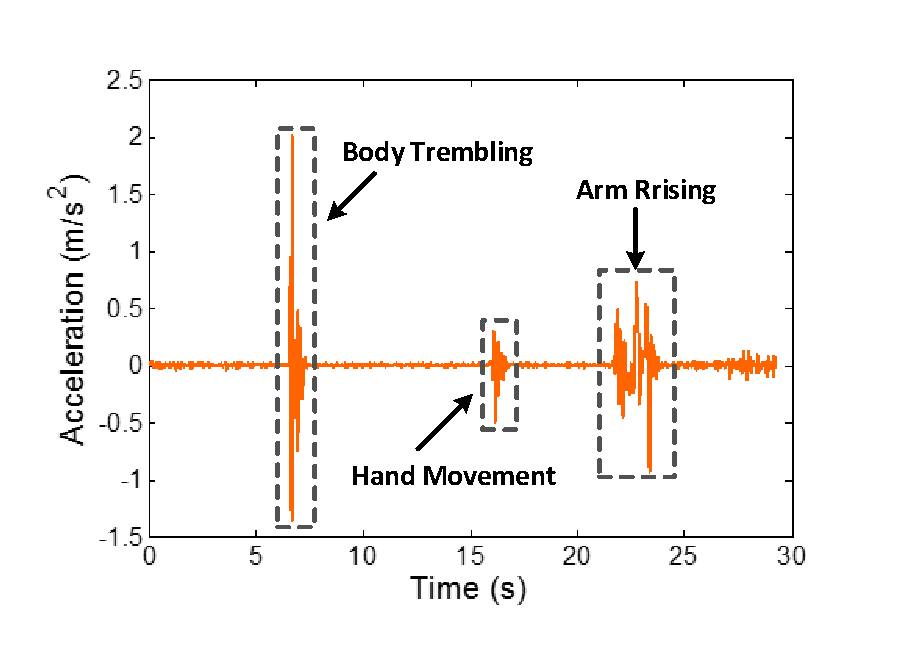
\includegraphics[width=0.77\linewidth]{Figures/Micromovement.pdf}
  \caption{Acceleration reading for micro body movements.}\label{fig:micro-move}
\end{figure}

For the two types of potential micro-movements to be classified, we calculate variances for 100 sets of micro-movement data for these 10 volunteers and perform peak detection, as well as make these peaks as features for a particular type of movement to establish a reference data set. In order to classify the micro-movement more accurately, we further obtain the average of the peak features in the reference data set. And then we determine the type of micro-movement with the smallest value of d as the final detection result.

%% �°�
\textcolor{blue}{\subsection{Acoustic Event}}
{\systemname} can also detect different acoustic events, which is another most important indicators of sleep quality. The snore, cough and somniloquy can suggest user's sleep quality and physical health. For example, snore is one of the possible symptoms of cerebral infarction patients. Different from traditional parameters based acoustic classification algorithm \cite{gu2016sleep}, we exploit the inherent characteristics of different acoustic events and design a lightweight algorithm for effective classification.

\begin{figure*}[!t]
\centering
%   \setlength{\abovecaptionskip}{-2pt}
% \setlength{\belowcaptionskip}{-9pt}
%\begin{minipage}[t]{0.32\linewidth}\centering
 \subfigure[Snore of six times.]{\label{snore}
   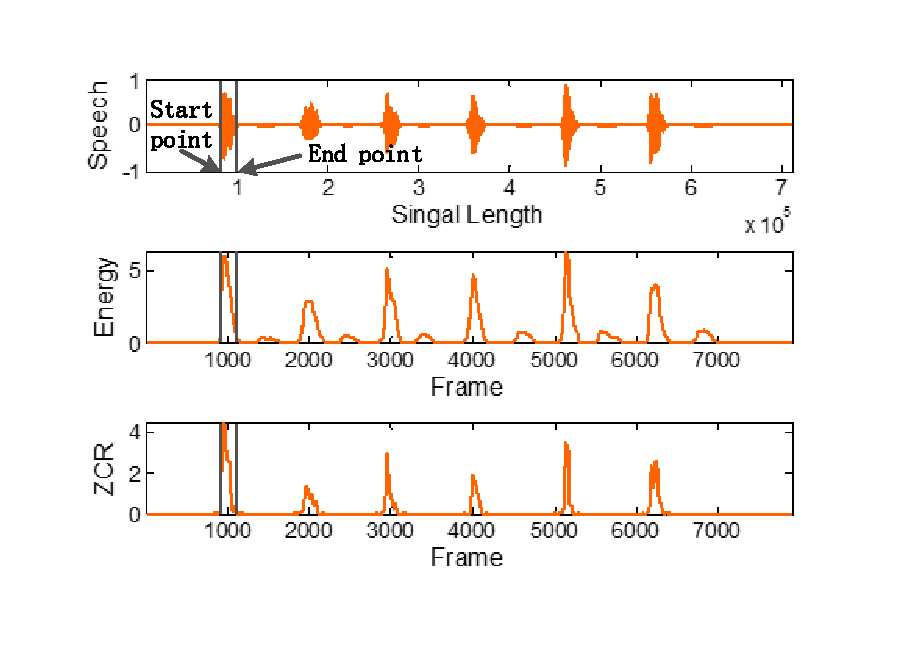
\includegraphics[width=0.325\linewidth]{Figures/snore.pdf}}
 \subfigure[Two consecutive cough.]{\label{cough}
   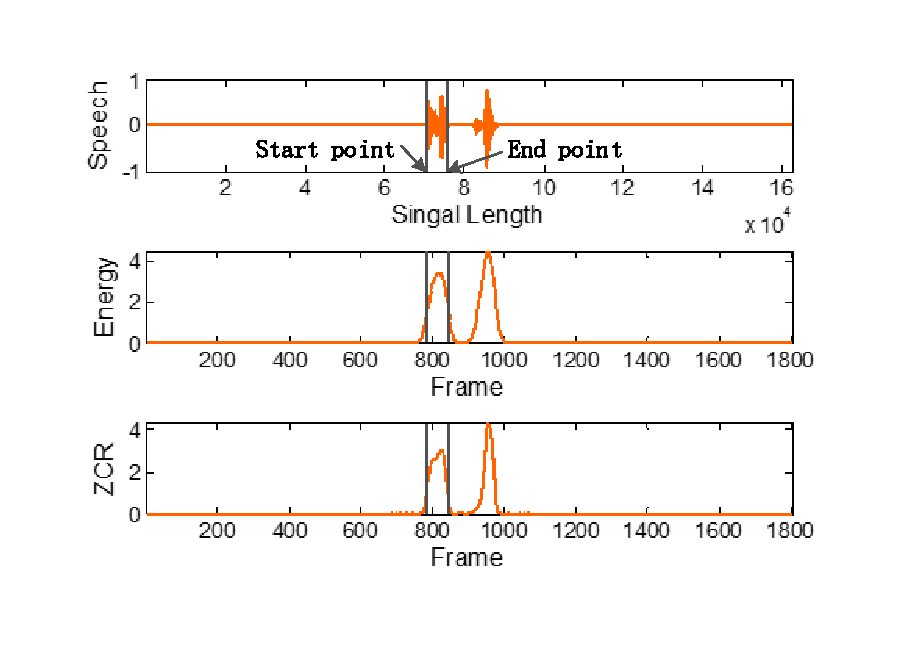
\includegraphics[width=0.325\linewidth]{Figures/cough.pdf}}
\subfigure[Somniloquy.]{\label{somniloquy}
     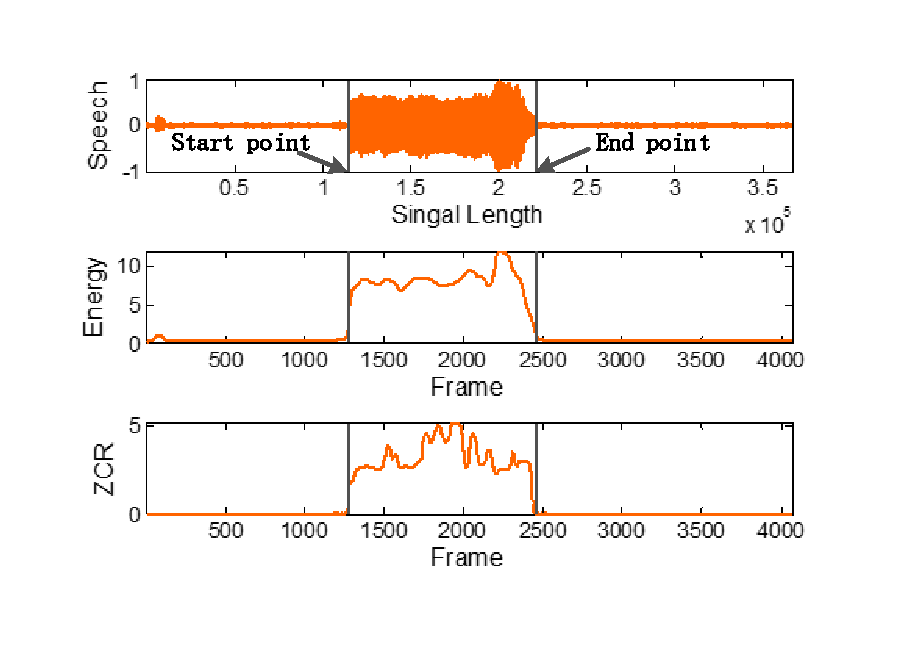
\includegraphics[width=0.325\linewidth]{Figures/somniloquy.pdf}}
\caption{The characteristics of different acoustic events.}\label{acoustic}
\end{figure*}


\textcolor{blue}{\subsubsection{Acoustic feature calculation}}
In order to identify different acoustic events accurately, we select the short-term average energy and the zero-crossing rate as two features. The short-term average energy of acoustic signal is computed as:
\begin{equation}
  E_i=\sum\nolimits_{j=-\infty}^{\infty}[x(j)\omega(i-j)]^2=\sum\nolimits_{j=i-(N-1)}^{i}[x(j)\omega(i-j)]^2,
\end{equation}
$N$ is the window length. As we can see that the short-term energy is the weighted sum of squared frame sample. The short-term energy can be used to distinguish the segment of unvoiced and voiced sound. It also can be used to differentiate speech segment and noise segment  in  case of relatively high signal to noise ratio (SNR). The zero-crossing rate is computed as:
\begin{equation}
  Z_i=\frac{1}{2}\sum\nolimits_{j=0}^{N}|sgn[x_i(j)]-sgn[x_i(j-1)]|.
\end{equation}
It indicates the number of times, which the acoustic signal waveform passes through the horizontal axis (zero level). We carry out an interesting recognition experiment using the microphone built in smartwatch to detect the sound of people during sleep and effectively identify different acoustic events. We focus on three common acoustic events: snore, cough and somniloquy. Ten volunteers worn the smartwatches during sleep to record the acoustic data. We manually label the data with different acoustic events. Fig. \ref{acoustic} shows the acoustic characteristics of  three events. There are six times snore event, two consecutive cough event and somniloquy event.
%The sample rate is 22050 Hz.


\textcolor{blue}{\subsubsection{Acoustic event recognition}}
 At beginning, the algorithm  divides the audio stream into frames with equal durations. Each frame is composed of 256 samples, and its duration is 12 ms. To identify the  three common acoustic events, we introduce an acoustic recognition algorithm based on the following key observations:

 \begin{itemize}[itemsep=1mm,nolistsep]
\item The time interval between two signals for different acoustic events are quite different from each other. As shown in Fig.~\ref{snore}, there is a long time interval between two snores. While, the time interval between two coughs is very short.  In contrast, the  somniloquy signal is irregular and without periodic property.
    %Besides, the snore event produces periodic signals and their intervals  are similar.
 \item The duration of one signal for different acoustic events are different from each other. Fig. \ref{acoustic} shows that the duration of a snore is shorter than the duration of a cough and somniloquy. And in general, the duration of a cough is shorter than the duration of a somniloquy signal.
\item The frequencies for different acoustic events are quite different from each other. Snore event has a continuous signal, while the  cough and somniloquy are sudden events, thus the number of consecutive occurrences is very small.
\end{itemize}
In conclusion, the ``interval'', ``duration'' and ``frequency'' of acoustic events can be used as three unique features. Based on the above three observations, our acoustic event recognition algorithm involves the following two steps. First, in order to estimate the interval and frequency of a acoustic event, we perform the peak detection. We use the short-term average energy to calculate the peak value of the acoustic signal. When the peak exceeds a certain threshold, such as 3 dB in this paper, we record the position of each peak and calculate the interval between two consecutive peaks. Next, we can estimate the frequency of a acoustic event by counting the number of peaks over a time window. Second, to estimate the duration of the acoustic event, we perform the start-point and end-point detection.

Traditional end-point detection algorithm \cite{stowell2015detection}, however, uses a fixed double threshold and must be obtained by a large number of data samples, which has two drawbacks. First, the fixed double threshold may cause error detection at the beginning of acoustic event. Second, the requirement of a large number of data samples would lead to large system latency. To deal with those problems, we introduce an improved end-point detection method, which improves the detection accuracy and reduces the number of data samples. The proposed method has a adaptive threshold, in detail, Since the first few frames and the last few frames are mostly mute or background noise, we select the first five frames and the last five frames to calculate their short-term energy, which are denoted as $Es$ and $Ee$, respectively. And then the two are combined to obtain the mean $En$ as the estimated energy value of the noise segment.Let the maximum value of the short-term energy over all frames denoted as $\max (E)$. Then, the average short-term energy $DE$ is given as:
\begin{equation}
      En=\frac{(Es+Ee)}{2},
\end{equation}
\begin{equation}\label{eq:DE}
      DE=\max (E)-En.
\end{equation}

So we can use $EH$ and $EL$ to represent the high and low threshold of short-term energy, which are given as:
\begin{equation}
      EH=0.1\times DE+En,
\end{equation}
\begin{equation}
    EL=0.06\times DE+En,
\end{equation}

 As a result, we can reduce the number of data samples required for detection. Moreover, in order to avoid the interference of sudden noise, we set the minimum length of the signal segment and count the length of the signal during the search for the start and end point. Finally, if the signal length is less than the set minimum, it is considered as a noise segment. The results of the start-point and end-point detection are shown in Fig. \ref{acoustic}, we calculate the length of each speech segment and calculate their averages as the duration of the acoustic event. Last, we count the number of peak points to determine whether it meets the third key observation or not.



%Algorithm 1 provides the detailed  process of the start-point  and end-point detections.


%$A_x$, $A_y$ and $A_z$ are the tilt angle of the three axes, and $\omega_x$, $\omega_y$ and $\omega_z$ are the rotation speed of the three axes. So $\phi$, $\theta$ and $\psi$ are the rotation angle of the three axes. \textcolor[rgb]{1.00,0.00,0.00}{(Those symbols do not present in Algorithm 1)}


%\begin{table}[!thbp]
%\begin{tabular}{l}
%  \hline
%  \textbf{Algorithm 1} The Endpoint Detection \\
%  \hline
%  \textbf{Input}: A sound signal recorded by the microphone:$x$
%  \\\quad \quad \quad The threshold of zero-crossing rate:$ZT$
%  \\\quad \quad \quad The minimum length of speech:$minlen$\\
%  \textbf{Output}:The start-point  and end-point :$p_s,p_e$\\
%  1: Split  $x$ using the framing algorithm \\
%  2: Calculate each frame of energy and zero-crossing rate:$E_i,Z_i$ \\
%  3: Calculate the threshold for short-time energy:$EH,EL$  \\
%  4:$count=0$,$silence=0$\\
%  \textbf{the start point}\\
%  5:\textbf{for}i=1$\rightarrow \frac{length(x)}{frame~length}$  do\\
%  6: \textbf{if} $ E_i>EH $ \textbf{then}\\
%  7: $count=count+1$,$silence = 0$,$max(n-count-1,1)=p_s$\\
%  8: \textbf{else if} $E_i>El || z_i>ZT $\textbf{then}\\
%  9: $count=count+1$ \\
%  10: \textbf{else}\\
%  11:$count=0 $ \\
%  12: \textbf{end if}\\
%  \textbf{the end point}\\
%  13:\textbf{if} $E_i>El || z_i>ZT $\textbf{then}\\
%  14:$count=count+1$ \\
%  15:\textbf{else}\\
%  16:$silence = silence+1 $ \\
%  17:\textbf{if} $count < minlen$\textbf{then}\\
%  18:$count=0 $, $silence=0$ \\
%  19:\textbf{end if}\\
%  20:$count1 = count-\frac{silence}{2}$\\
%  21:$ p_e = p_s + count1 -1$ \\
%  \hline
%\end{tabular}
%\end{table}


\textcolor{blue}{\subsection{Illumination Condition}}
Studies have shown that there is a significant interaction between illuminance level and the mental state of the individual \cite{light77}. For example, the bright light can counteract subjective fatigue during daytime, but at night it will make it difficult to fall asleep and seriously affecting the sleep quality. Thus we use the ambient light sensor to detect the illumination condition during sleep. We visit 10 volunteers' bedroom at night and the use of the ambient light sensor to test the lighting conditions in the bedroom, and ultimately we will divide the illumination intensity into two conditions: bedroom without light (Weak illumination condition, $\leq$ 10Lux);  bedroom with strong lights (Strong illumination condition, $>$ 10Lux). Therefore, we can learn the light conditions in the sleeping environment according to the two types of illumination conditions.

However, the light sensor may be obscured, which leads to large errors in measuring the illumination level. For example, a user��s smartwatch may be covered under quilt when he/she turned over unconsciously, and thus the illumination readings on the smartwatch may not reflect the real lighting situation. To deal with this problem, the key is that the illumination would drop suddenly when the smartwatch is covered by other objects. There are two possibilities for the sudden drop in light intensity. For most smartwatches, the light sensors are usually installed in the front face of it. The first case is the indoor lighting facilities are closed. The second case is the wrist turned so that the back of the hand become downward, thus blocking the light sensor in front of the smartwatch. To avoid this erroneous illumination condition measurement, we detect whether the user is performing a wrist flip over a period of time during the intensity plummeting. We detect the wrist flip based on two aspects: (i) the rotation angle of smartwatch; (ii) wether the light intensity maintain stable after the sharp drop. If the wrist flips, we use the average of the previous light intensity as the intensity of the time period.

\textcolor{blue}{\subsection{Sleep stage and quality}}
Sleep is a cyclical process composed of three stages: rapid eye movement (REM) stage, light sleep stage and deep sleep stage. The entire sleep process can be divided into many sleep cycles, in each sleep cycle, the sleeper first experienced a transition from light sleep to deep sleep, and then enter the REM. However, the sleep stage can also jump from light sleep to REM or deep sleep directly from REM.To estimate the sleep stage, we use the HMM model \cite{johnson2010hidden} since different sleep stages have potential conversion probabilities. Usually, when a user is in different sleep stages, he/she will have different sleep-related activities.For example, a person may roll over in bed when he/she is in light sleep stage, and keep motionless when he/she is in deep sleep stage. And when he/she get into the deep sleep, it will appear snoring, body trembling, etc., in the meanwhile, the breathing amplitude larger than when he/she sleep in the light stage. Thus, based on these features,we use all the detected sleep-related activities as the HMM model input. And we use a series of sleep events as observation sequence, corresponding to the sleep stage as an implicit state sequence, first using maximum likelihood estimation method for parameter estimation, the state transition matrix and the confusion matrix, and then use the Viterbi algorithm \cite{viterbi} can be obtained A series of implicit state sequences corresponding to observed sequences. That is to say that  based on HMM model, we can estimate the sleep stage during a time window, such as 2 hours. Finally, we can get the durations of all sleep stage over the whole sleep process.

Further, to quantize the quality of a sleep, we use the Sleep Quality Report model introduced in \cite{gu2016sleep}. Let $SQ$ be the value of the sleep quality, then $SQ$ is given as follow:
 \begin{equation}
SQ=\frac{(REM \times 0.5+Light \times 0.75+Deep) \times 100}{REM+Light+Deep}
 \end{equation}
where, REM, Deep and Light represents the duration time in a sleep process. The range of $SQ$ is from 50 to 100. A high value of $SQ$ shows a good  sleep quality.
% In order to better analyse the sleep patterns, we detect the ambient illumination conditions in the sleep environment. We have carried out the experiments many times in  different indoor environments and different lighting conditions. The experiments can be divided into two categories: bedroom with dim light (Weak illumination condition, $\leq$10 Lux); bedroom with strong light (Strong illumination condition, average of 180 Lux).  Therefore, we can utilize the light sensor built in smartwatch to measure different light condition that will be a part of sleep pattern.
